\chapter{研究现状综述}\label{chap:relatedwork}

% 2.1 引言
\section{引言}
% 任务背景
% 可以介绍统计机器翻译到神经机器翻译的变革,带来了哪些影响,例如在多模态融合等方面的影响
机器翻译是一种利用计算机算法将一种语言翻译到另一种语言的技术。从统计机器翻译时代,到神经机器翻译时代,机器翻译相关技术一直作为行业的风向标引领着整个自然语言处理领域的发展。其基础模型从做到打破语言壁垒突破至跨越模态整合,能够在计算机视觉、语音信号处理以及多模态信息融合等领域都得到广泛的应用。
% 任务起源
% 可以提到机器翻译的缺陷,比如歧义、信息不充足等问题试图通过外源信息来解决
多模态机器翻译就是一种在机器翻译的基础上,融合图像信息、语音信息或者视频信息的一类方法。这些引入的外源信息,在理论上具有解决歧义词、转录错误以及语义不完整等问题的意义。

% 任务形式
% 讲讲与机器翻译的区别、如何将其分为了两大类。
融合图片信息的神经机器翻译是多模态神经机器翻译方法的一个分支,是一种将图片作为外源辅助信息输入到神经机器翻译模型中,以提升翻译准确率为目的的方法。因此,与常规的神经机器翻译相似的是,相关研究所使用的语料同样需要平行翻译句对的形式,区别在于增加了与文本内容高度相关的图片输入。根据图片信息的作用方式,可以将相关方法分为图片信息辅助式、图片信息增强式、图片搜索式以及无监督式的四类方法。本章首先将简要介绍神经机器翻译的发展过程,以及用于对图片进行预处理以及特征提取的计算机视觉基础模型,然后按照图片信息辅助式、图片信息增强式、图片搜索式和无监督式的方法分类,分别介绍融合图片信息的神经机器翻译如何随着神经机器翻译的发展而进行改进。

% 2.2 神经机器翻译
\section{神经机器翻译模型}
\label{sec:2_nmt}
在融合图片信息的神经机器翻译中,平行翻译句对的源语言句子与目标语言句子之间一般具有很强的语义对齐关系,而图片主要起到补充信息的作用。因此,ImgNMT所使用的模型多数是以神经机器翻译模型作为基础框架,视觉特征作为模型的额外输入。本节将介绍ImgNMT在模型设计发展过程中所应用到的神经机器翻译基础模型框架,这其中包含:基于循环神经网络(recurrent neural network,RNN)方法的神经机器翻译(RNN-based neural machine translation,RNMT)模型\pcite{sutskever2014sequence,cho2014learning}、增加注意力机制的RNMT模型\pcite{bahdanau2015neural,luong2015effective}以及基于自注意力机制的Transformer\pcite{vaswani2017attention}。另外,还有基于卷积神经网络(convolutional neural networks,CNN)的NMT模型\pcite{gehring2017convolutional},但其很快被自注意力机制取代,也没有在ImgNMT任务上得到应用,因此本节忽略这部分内容的介绍。

\subsection{循环神经网络}
\label{sec:2_rnn}
\begin{figure}[!htbp]
    \centering
    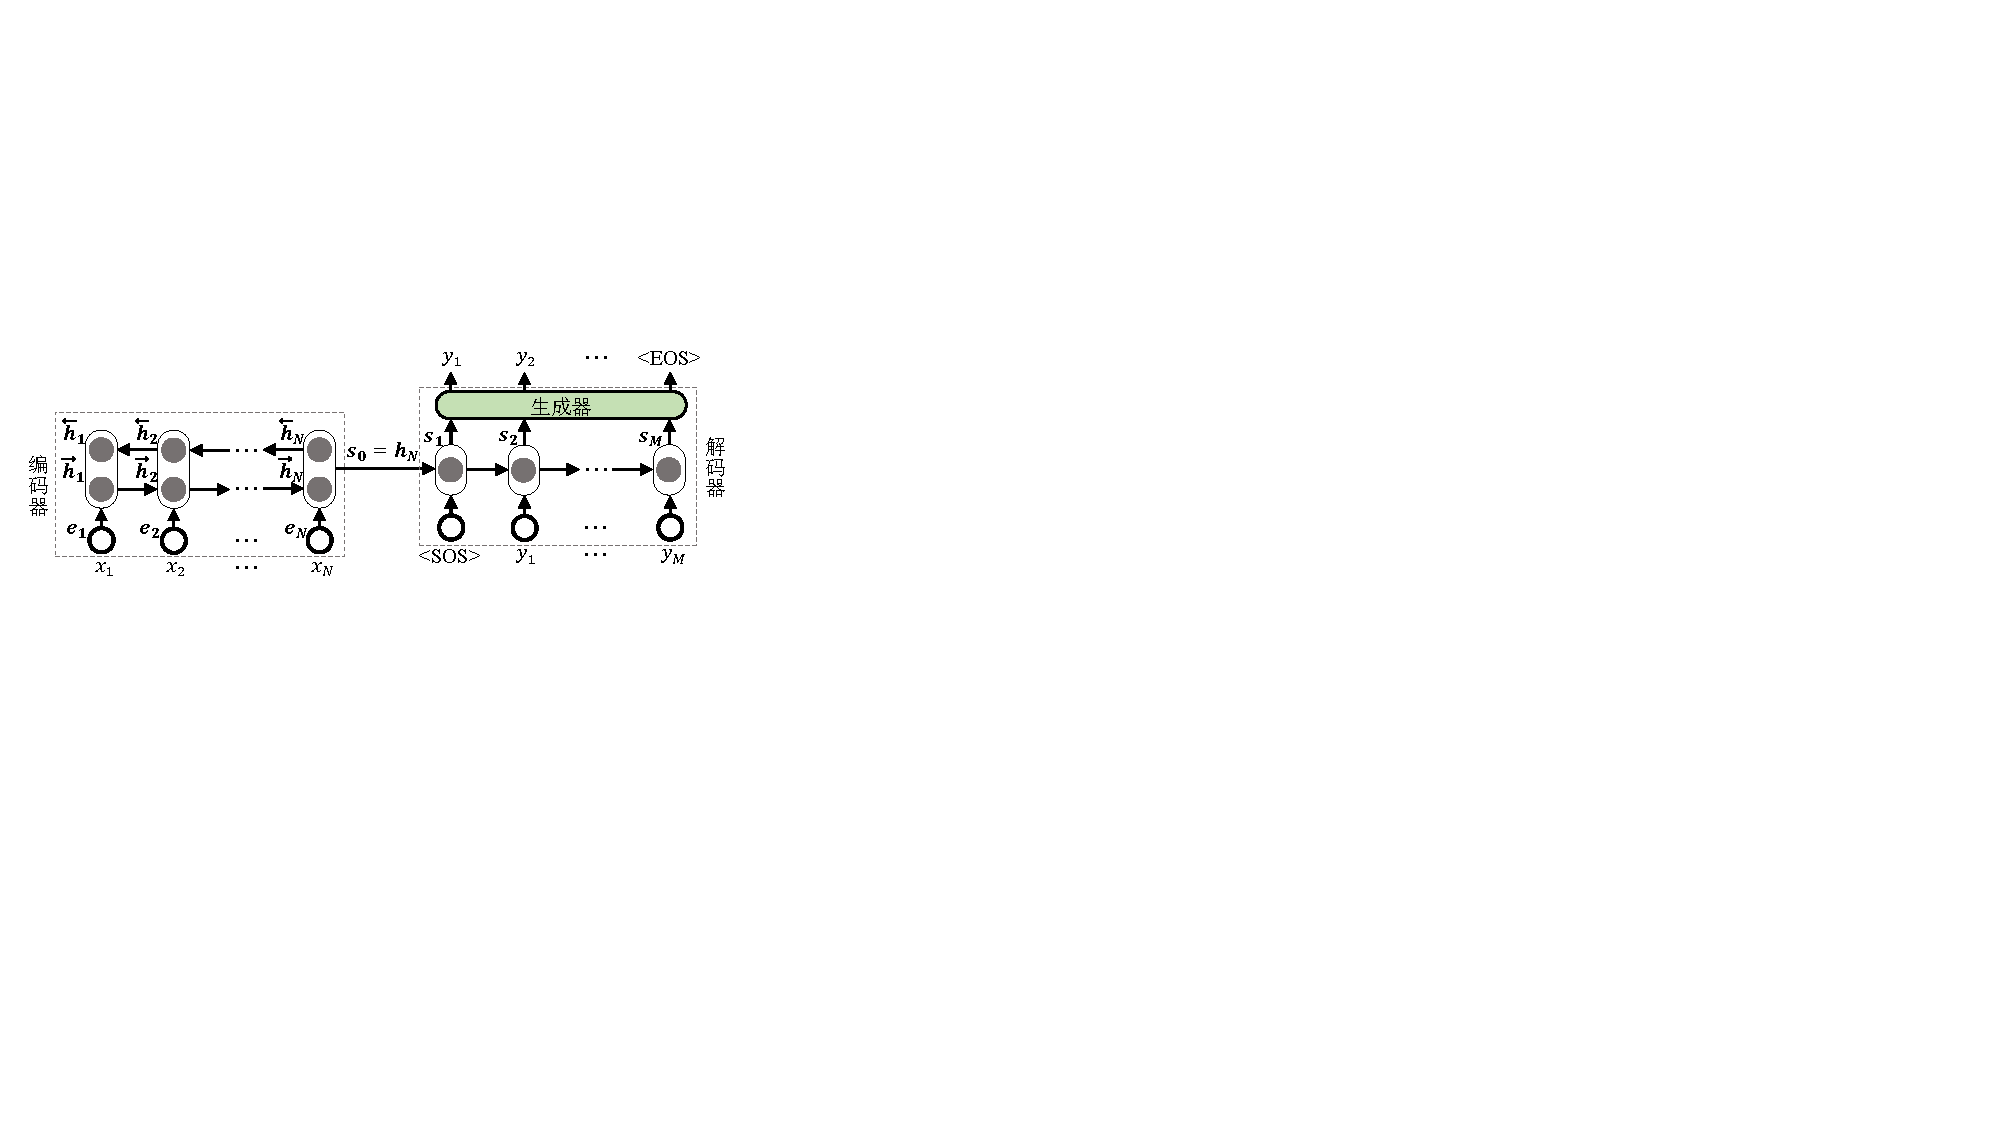
\includegraphics[scale=1]{Img/fig_2_rnmt.pdf}
    \bicaption{基于循环神经网络的神经机器翻译}{Neural machine translation based on recurrent neural network}
    \label{fig:2_rnmt}
\end{figure}
神经机器翻译是一种序列到序列的生成任务,其源端序列与目标端序列的长度往往是不同的。因此,编码器-解码器结构成为了神经机器翻译的常用模型框架。编码器和解码器分别用于编码源端序列和解码到目标端序列。循环神经网络就是一种用于解决序列建模的方法。图\ref{fig:2_rnmt}为基于循环神经网络的神经机器翻译框架。编码器将不定长的源语言句子编码为单个固定维度的隐层向量,该隐层向量可作为整个句子语义的特征表示。解码器负责根据该特征表示生成目标语言句子。形式化地,给定待翻译的源语言句子$X=\{x_1,x_2,…,x_N\}$,在编码端首先需要将$X$中的词转化为词向量$E=\{\Vector{e_1,e_2,…,e_n}\}$,其中:
\begin{equation}
    \Vector{e_i}=\mathrm{Emb}(x_i)
\end{equation}

源语言句子中的每个词$x_i$均有一个对应的词向量表示$\Vector{e_i}$。然后编码器按照句子中词的顺序将句子编码到一个隐层状态序列$\rarwvec{H}={\rarwvec{h}_1,\rarwvec{h}_2,…,\rarwvec{h}_N}$,其中,$\rarwvec{h}_i$中编码了输入序列中前$i$项的信息,即:
\begin{equation}
    \rarwvec{h}_i=\mathrm{RNN}(\rarwvec{h}_{i-1},\rarwvec{e}_i)
\end{equation}
其中$\rarwvec{h}_{0}$可随机初始化或置为零向量。为了使每个位置的编码都能融合整个输入序列的信息,可采用双向编码器将句子$X$同时编码到$\rarwvec{H}$和$\larwvec{H}$,其中,$\larwvec{H}=\{\larwvec{h}_1,\larwvec{h}_2,…,\larwvec{h}_N\}$为$X$的逆序编码结果,即:
\begin{equation}
    \larwvec{h}_i=\mathrm{RNN}(\larwvec{h}_{i+1},\larwvec{e}_i)
\end{equation}
将$\rarwvec{H}$和$\larwvec{H}$拼接得到$\Vector{H=\{h_1,h_2,\cdots,h_N}\}$, 其中:
\begin{equation}
    \Vector{h_i}=[\rarwvec{h}_i;\larwvec{h}_i]
\end{equation}

RNMT的解码器同样采用循环神经网络生成目标语言文本。该生成翻译的过程是自回归的,即在时刻$t$,解码器需要根据$0$至$t-1$时刻的解码结果及源语言所提供的上下文信息进行当前时刻的预测结果的生成:
\begin{equation}
    \Vector{s}_t=\mathrm{RNN}(\Vector{s_{t-1}},y_{t-1})
\end{equation}
\begin{equation}
    P(y_t|y_{<t},X)=\mathrm{softmax}(g(\Vector{s_t}, y_{t-1}, \Vector{c_t}))
\end{equation}
该过程中,源端上下文信息的作用方式有很多种。\tcite{sutskever2014sequence}将$\rarwvec{h}_N$传递给解码器作为初始状态$\Vector{s_0}$。\tcite{cho2014learning}将$0$至$t-1$时刻的解码结果编码,并连同源端上下文信息$\Vector{H}$预测当前时刻单词:
\begin{equation}
    \Vector{c_t}=f(\Vector{H})
\end{equation}
其中,$f(\cdot)$表示选用平均池化(average pooling)对$\Vector{H}$取平均,或直接选取$\Vector{H}$的最后一项$\Vector{h_n}$。

虽然基于循环神经网络的神经机器翻译还没有实现对传统统计机器翻译在翻译准确率上的全面超越,但其采用的编码器-解码器框架已经展现了能够将文本数据进行分布式表示并从这种表示中解码到目标语言译文的能力。这种分布式表示方法也为跨模态信息的融合提供了极大的便利。

\subsection{注意力机制}
\label{sec:2_attention}
基于编码器-解码器结构的神经翻译模型利用编码器将源语言编码为一个固定的特征向量,再利用解码器中的循环神经网络编码已生成的目标端单词,从而指导新的目标端单词的生成。在该过程中,编码的源语言特征向量作为句子级语义的完整表示,一方面丢失了源语言中的句长信息,另一方面无法指导在当前时刻$t$生成目标端单词时应该更多地关注源端的哪些信息。为了解决这个问题,\tcite{bahdanau2015neural}提出在编码器与解码器之间增加注意力机制(attention mechanism)。

\begin{figure}[!htbp]
    \centering
    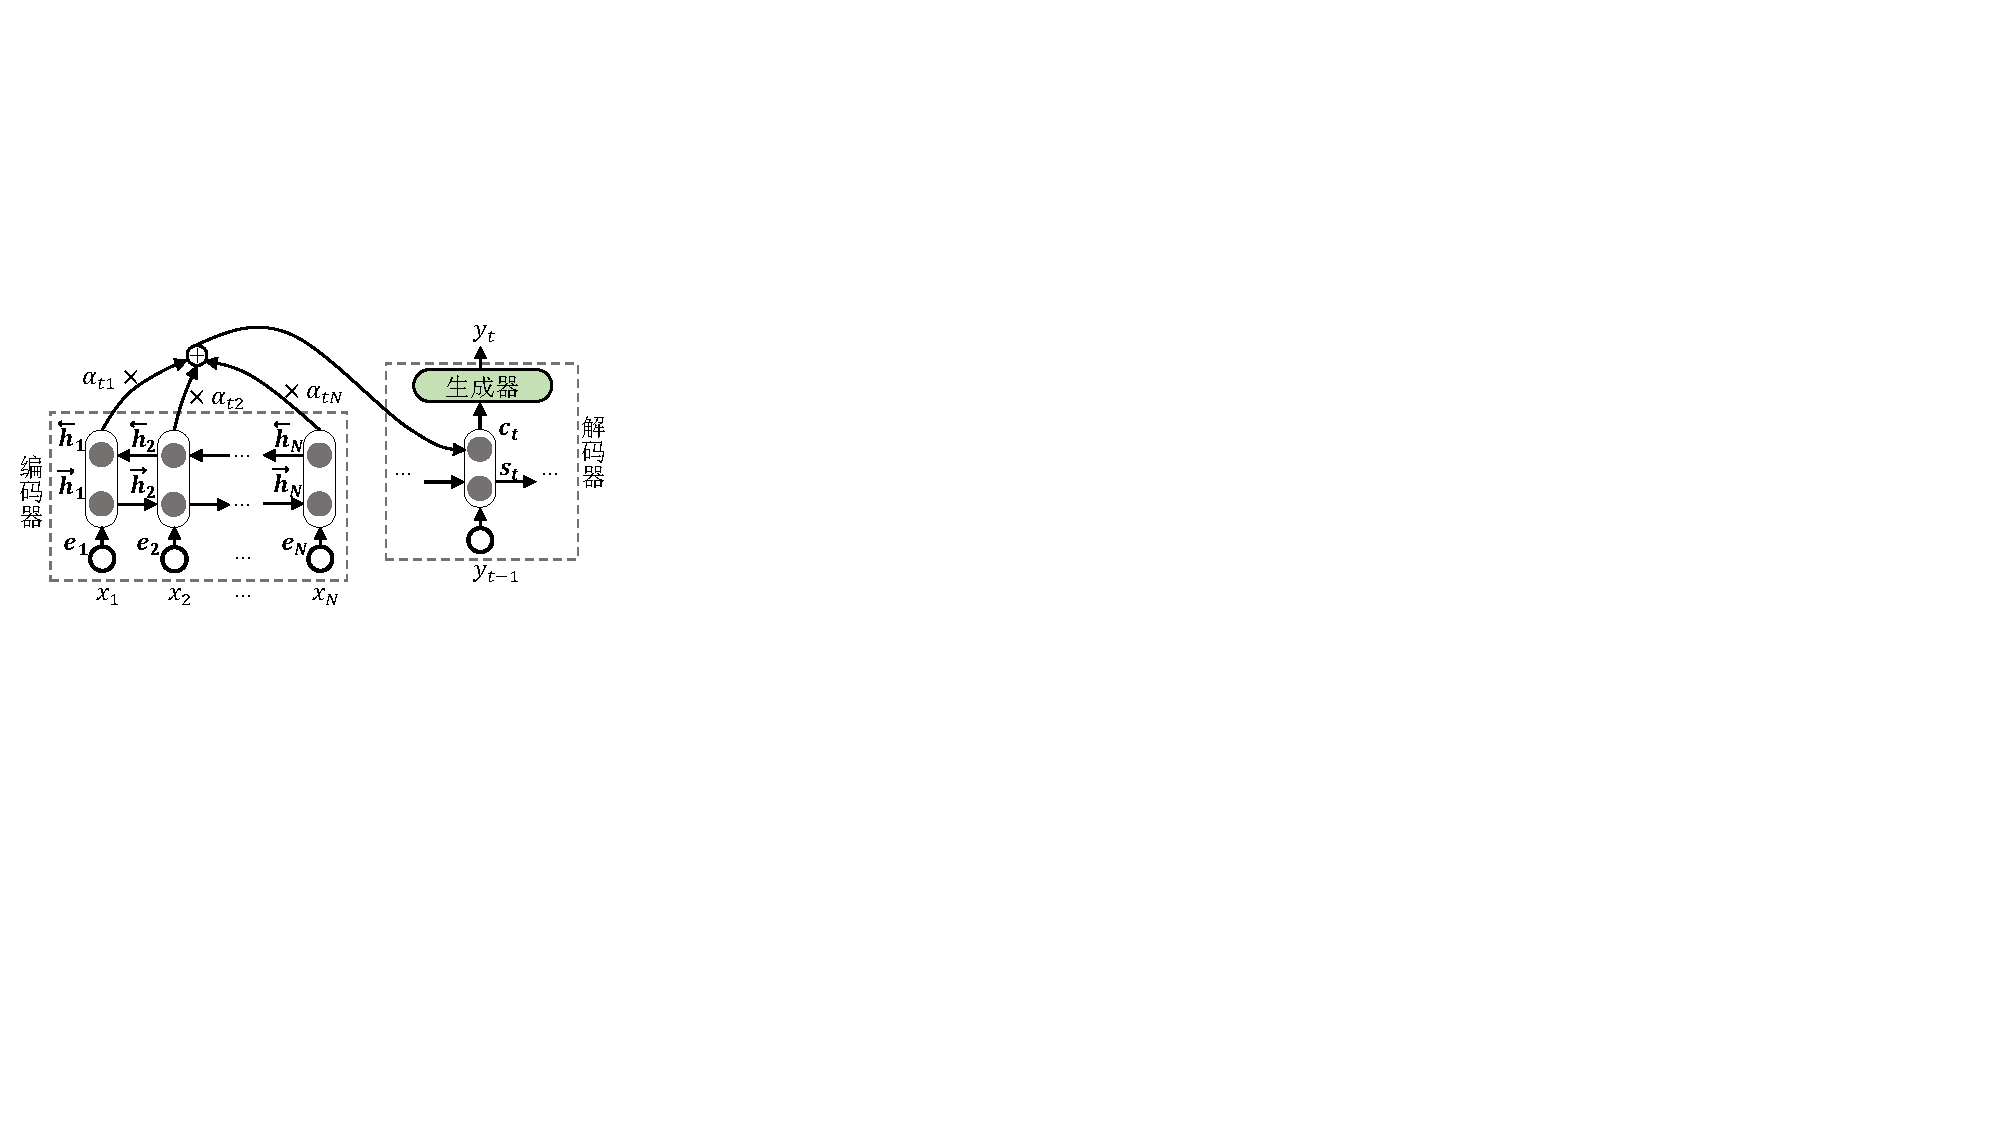
\includegraphics[scale=1]{Img/fig_2_att_rnmt.pdf}
    \bicaption{增加注意力机制的RNMT}{Attention-based RNMT}
    \label{fig:2_att_rnmt}
\end{figure}
图\ref{fig:2_att_rnmt}为增加了注意力机制的神经机器翻译,其编码器和解码器保留原来的工作方式,而两者之间的注意力模块为解码器提供了动态的源语言上下文信息。对于每个时刻$t$,源语言上下文向量$\Vector{c_t}$由固定的特征向量替换为与$t$相关的表示:
\begin{equation}
    \Vector{c_t} = f_t(\Vector{H})=\sum_{i=1}^{N}{\alpha}_{ti}\Vector{h_i}
\end{equation}
\begin{equation}
    {\alpha}_{ti}=\frac{\mathrm{exp}(a_{ti})}{\sum_{j=1}^{n}\mathrm{exp}(a_{tj})}
\end{equation}
\tcite{bahdanau2015neural}所提方法中:
\begin{equation}
    a_{ti} = \mathrm{score}(\Vector{s_{t-1},h_i})
\end{equation}
其中$\mathrm{score}(\cdot)$是打分函数,计算两个向量所携带信息的相关程度,可采用点积或多层感知机等方法。上式对$\Vector{s_{t-1}}$和$\Vector{h_i}$进行打分,表示根据已生成的目标文本编码表示$\Vector{s_{t-1}}$,计算源语言中第$i$项对当前时刻$t$的重要程度。因此,$a_{ti}$代表着生成$t$时刻的目标端单词时,对源语言中第$i$项的“关注”度,${\alpha}_{ti}$就是该“关注”度的归一化结果,$\Vector{c_t}$就是根据“关注”度对特征向量的加权表示。

值得注意的是,$t-1$时刻的输出结果$y_{t-1}$是由$\Vector{s_{t-1}}$得到的,因此上式中丢失了$y_{t-1}$的信息,\tcite{luong2015effective}提出了改进方案:
\begin{equation}
    a_{ti} = \mathrm{score}(\Vector{s_{t},h_i})
\end{equation}
并规定了$\mathrm{score}(\cdot)$的三种计算方式,综合\tcite{bahdanau2015neural}等提出的方法,可得到以下四种方法:
\begin{equation}
    \mathrm{score}(\Vector{s_t, h_i}) = 
    \begin{cases}
        \Vector{s_t^T h_i} & \mbox{{\itshape 点积法}} \\
        \Vector{s_t^T W_a h_i} & \mbox{{\itshape 通用点积法}} \\
        \Vector{W_a[s_t; h_i]} & \mbox{{\itshape 连接法}} \\
        \Vector{v_a^T} \mathrm{tanh}(\Vector{W_a s_t+U_a h_i}) & \mbox{{\itshape 多层感知机法}} 
    \end{cases}
\end{equation}
其中$\Vector{v_a}$、$\Vector{W_a}$和$\Vector{U_a}$是网络参数,$T$表示对向量进行转置。

%(注意力机制在视觉领域的应用,以及在跨模态领域的应用。)

\subsection{Transformer}
\label{sec:2_transformer}
\begin{figure}[!htbp]
    \centering
    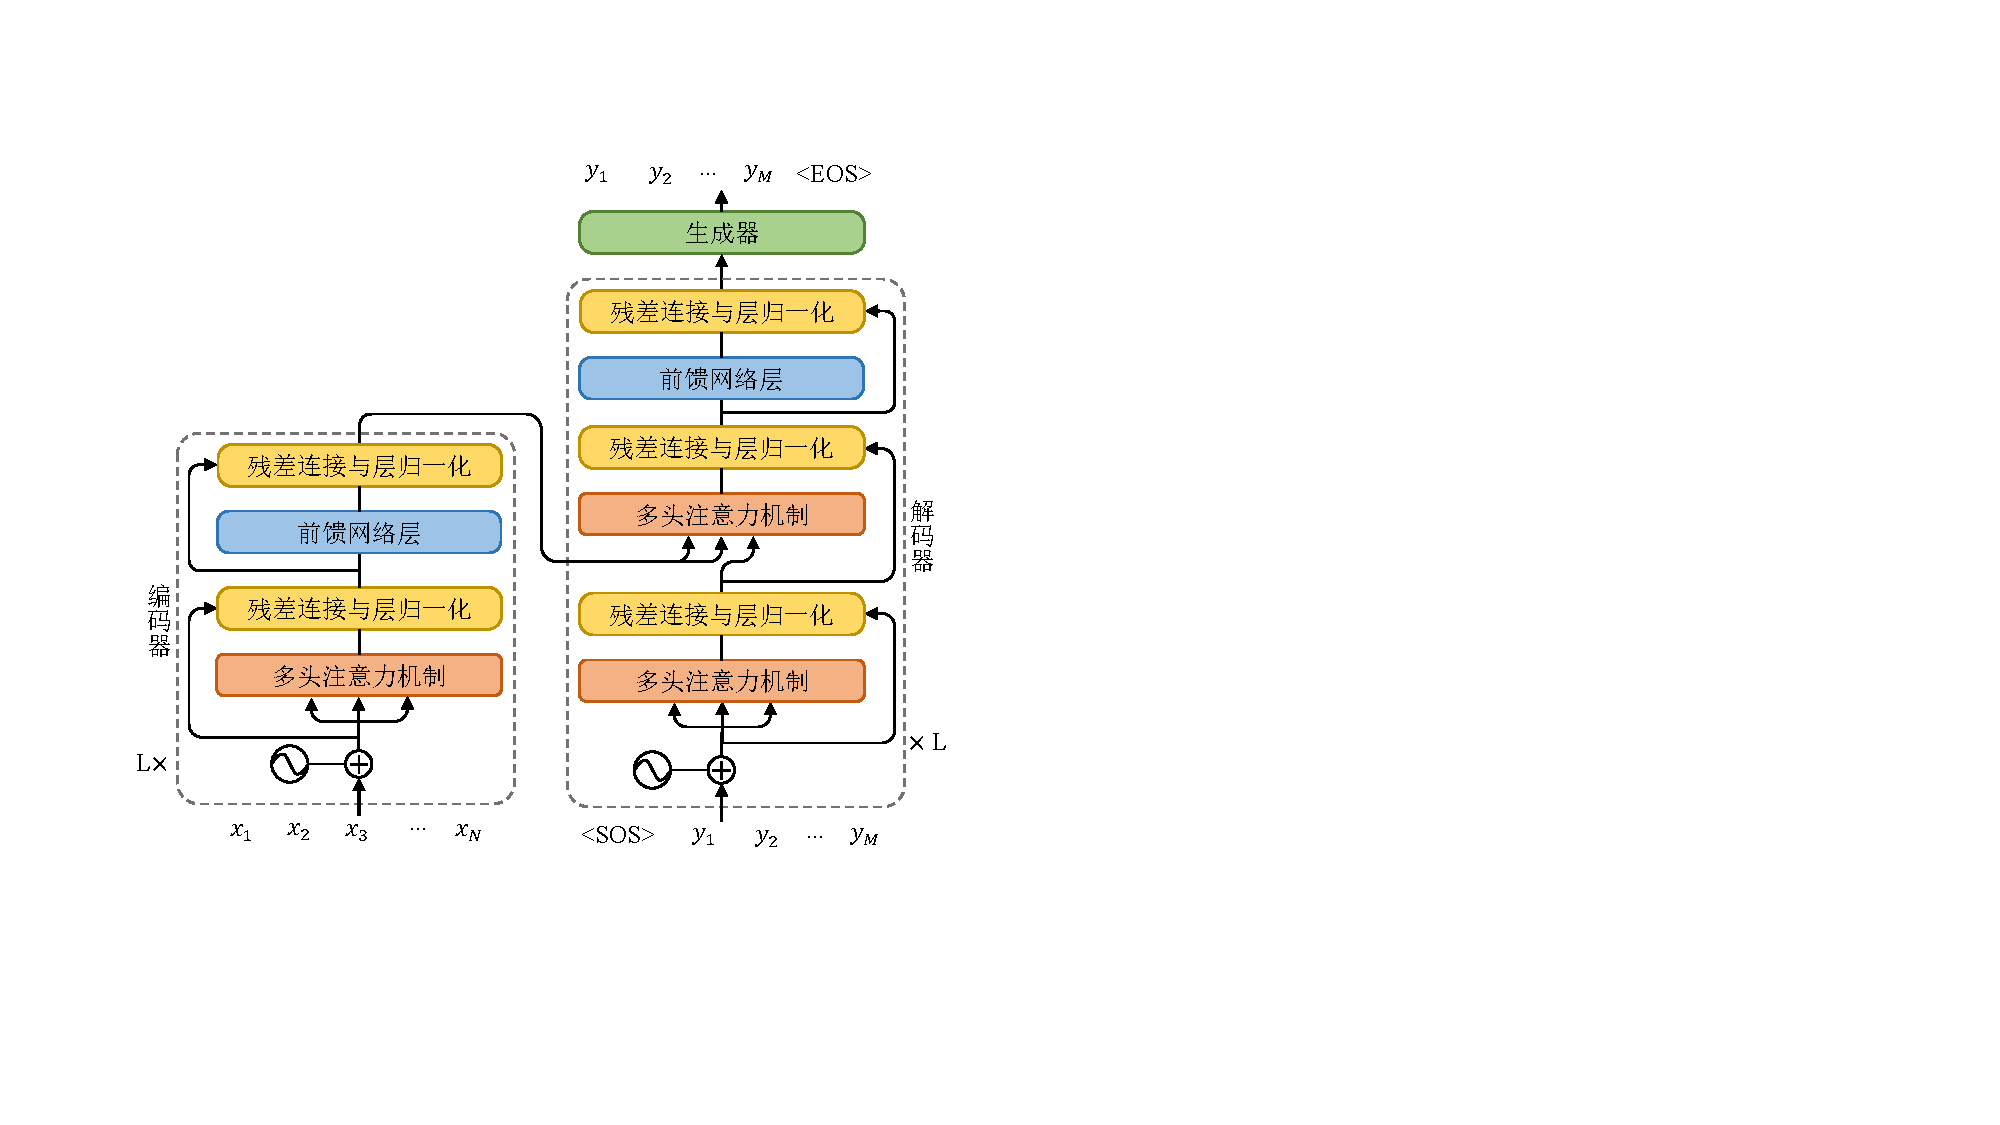
\includegraphics[scale=1]{Img/fig_2_transformer.pdf}
    \bicaption{基于Transformer的神经机器翻译}{Transformer-based neural machine translation}
    \label{fig:2_transformer}
\end{figure}
在注意力机制的帮助下,基于循环神经网络的神经机器翻译得到了显著的性能提升。这说明基于动态上下文的解码方法能够更准确地捕捉上下文信息,从而得到更忠于原文的译文。而注意力机制相当于二次编码,为下游模块提供动态上下文。既然注意力机制同样具有编码能力,那么是否可以用于替换循环神经网络呢?谷歌提出的Transformer\pcite{vaswani2017attention}就是一种基于这种假设的模型。图\ref{fig:2_transformer}展示了Transformer的模型结构,其保留了编码器-解码器的基础框架,利用内置的多头注意力机制(multi-head attention mechanism)实现编码与解码过程。


\begin{figure}[!htbp]
    \centering
    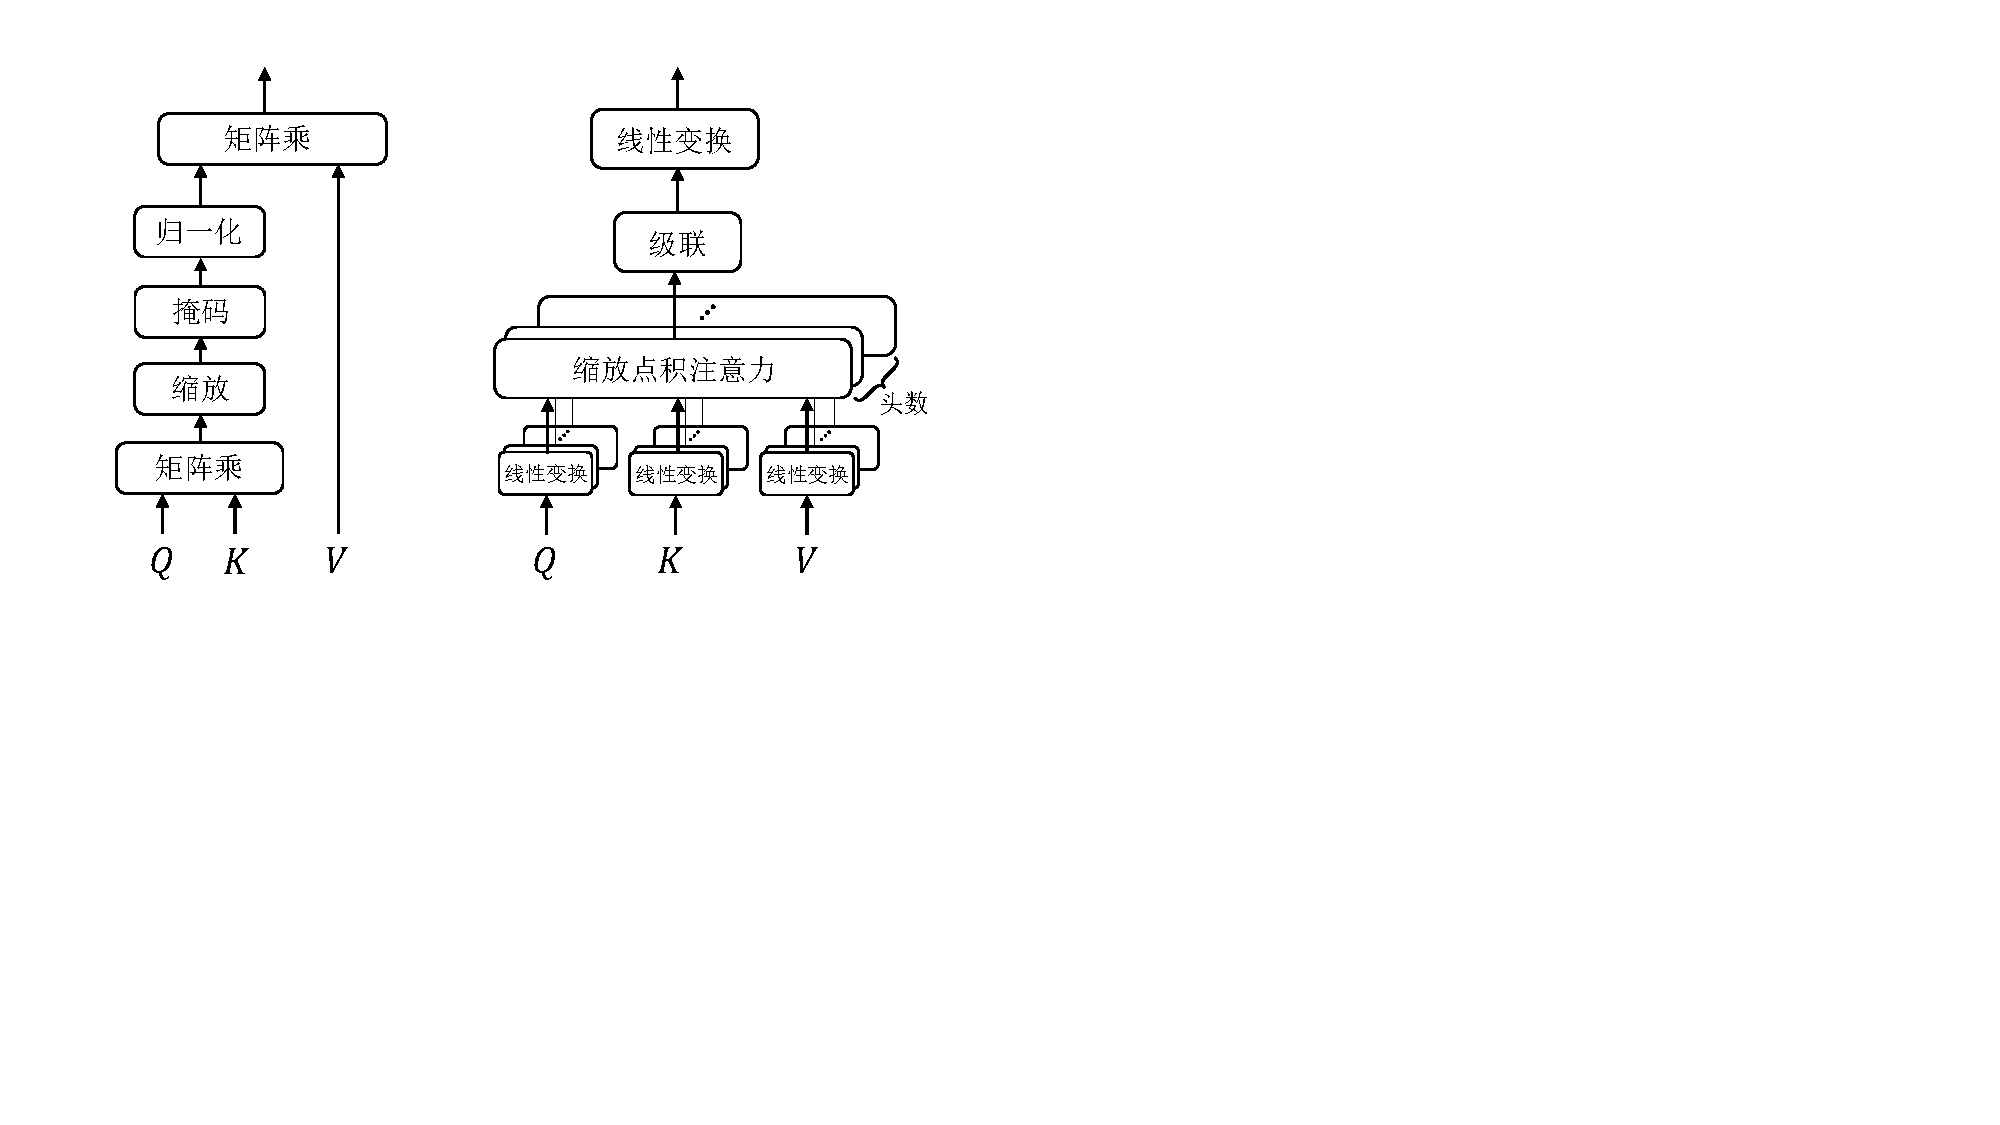
\includegraphics[scale=0.8]{Img/fig_2_multihead.pdf}
    \bicaption{多头注意力机制框架图}{Frame diagram of multi-head attention mechanism}
    \label{fig:2_multihead}
\end{figure}
区别于一般的注意力机制,多头注意力机制采用了一种更具泛化性的模型设计。如图\ref{fig:2_multihead}所示,多头注意力机制的输入分为查询(query,Q)、键(key,K)以及值(value,V)三部分,并结合了缩放点积注意力(scaled dot-product attention)和多头注意力(multi-head attention)两种方法。

{\sffamily 缩放点积注意力:}与一般的点积法相比,缩放点积注意力增加了一个缩放因子$d_k^{-0.5}$:
\begin{equation}
    \mathrm{Attention}(\Vector{Q},\Vector{K},\Vector{V}) = \mathrm{softmax} \left( \frac{\Vector{Q}\Vector{K}^T}{\sqrt{d_k}} \right) \Vector{V}
\end{equation}
其中,$d_k$代表$\Vector{Q}$、$\Vector{K}$和$\Vector{V}$的隐层维度。采用点积法的优点在于点积是以矩阵乘的形式进行计算,通过底层代码优化等方法可以很好地对矩阵乘进行硬件加速。引入缩放因子则是为了防止$d_k$较大时,点积的数值膨胀导致$\mathrm{softmax}(\cdot)$函数逼近梯度消失的数值范围。

{\sffamily 多头注意力:}为了丰富动态上下文所承载的信息,\tcite{vaswani2017attention}将多个注意力模块拼接组成多头注意力机制:
\begin{equation}
    \mathrm{MultiHead}(\Vector{Q,K,V}) = \mathrm{Concat}(\Vector{head_1, \cdots, head_n})\Vector{W^O}
\end{equation}
\begin{equation}
    \Vector{head_i} = \mathrm{Attention}(\Vector{Q W_i^Q,K W_i^K,V W_i^V})
\end{equation}
其中,$\Vector{W_O}$,$\Vector{W_i^Q}$,$\Vector{W_i^K}$和$\Vector{W_i^V}$是模型参数。$\Vector{Q}$、$\Vector{K}$和$\Vector{V}$经过不同的参数映射到不同的表示空间,再由注意力机制编码得到的不同的上下文特征表示。该过程相当于在不增加额外参数的情况下,将多个模型集成到一个模型中,从而提升模型的学习能力。

多头注意力机制在Transformer中的用途分为三种:
\begin{itemize}
    \item 位于编码器的多头自注意力机制用于编码源语言句子,此时Transformer编码器第一层的$\Vector{Q}$、$\Vector{K}$和$\Vector{V}$均为源语言句子经映射后的词向量序列,其它层的$\Vector{Q}$、$\Vector{K}$和$\Vector{V}$为前一层的输出。
    \item 位于解码器中带有掩码的多头自注意力机制用于编码目标端已经解码出来的部分句子。掩码的作用是为了保持自回归解码过程中后面位置单词的解码只能用到前面位置信息的特性。
    \item 连接编码器与解码器的多头交叉注意力机制的作用和一般的注意力机制相似。此时$\Vector{Q}$为解码器中带有掩码的多头自注意力机制的输出,$\Vector{K}$和$\Vector{V}$为编码器的隐层输出。交叉注意力机制输出的是融合了源端信息的目标端句子的表示。
\end{itemize}

值得注意的是,基于注意力机制的编码过程与循环神经网络相比丢失了对输入序列位置信息的建模。因此,\tcite{vaswani2017attention}提出了位置编码(positional encoding),为每个词向量增加位置信息。%文献\cite{DBLP:journals/corr/GehringAGYD17}则提出了更为方便的位置词向量的方案。

尽管近年来针对Transformer框架的改动层出不穷,但广泛应用的模型基本保持了最原始的设计方案。常见的改动如\tcite{devlin2019bert}提出了使用位置词向量(positional embedding)的方式替换位置编码,以及为了加强Transformer对长序列的编码能力提出相对位置编码\pcite{shaw2018self,dai2019transformerxl}。而这些创新性的改动基本都保留了Transformer中的自注意力机制和交叉注意力机制的基本结构。除了机器翻译等生成式任务外,在大规模预训练任务的表现上,Transformer更是充分展现了其应用场景的灵活性\citep{radfordimproving,devlin2019bert,liu2019roberta,lewis2020bart,raffel2020exploring}。针对不同规模的数据,通过增减参数规模的方式就可以使其适应相应的任务。相比于基于循环神经网络的模型,Transformer能够容纳更长的输入序列和更大规模的网络参数。

Transformer出色的编码能力不仅在自然语言处理任务大放异彩,还在计算机视觉以及多模态信息融合等领域展现了不俗的潜能。例如在计算机视觉领域的图像分类、目标检测以及语义分割等传统任务上摒弃了基于卷积神经网络的方法,直接采用Transformer作为基础模型,并在多个任务上得到了进一步的性能提升\pcite{parmar2018image,dosovitskiy2021vit,liu2021swin,yuan2021tokens};或是在大规模文本预训练模型的基础上,在输入序列中增加图片输入或从图片中提取的视觉目标,提升Transformer在多模态自然语言理解(multi-modal natural language understanding)任务上的能力\pcite{lu2019vilbert,chen2020uniter,huang2020pixelbert,kim2021vilt}。

%(Transformer已经在业界产生的影响力,自注意力替换循环神经网络的必要性,解决了哪些问题)

% 2.3 visual backbones
\section{计算机视觉基础模型}
\label{sec:2_cv}

深度学习技术不仅推动着自然语言处理技术的发展与革命,其在早期更是在计算机视觉领域推动各项技术从研究起步迈向成熟落地。相比于自然语言处理技术在近年来才迎来应用热潮,计算机视觉中的相关研究则早已应用到生产生活中。这也是目前大部分融合视觉信息的自然语言处理任务均应用预训练好的计算机视觉基础模型对图像进行编码的原因。

融合图片信息的神经机器翻译任务需要将图片信息输入到神经机器翻译模型中,因此同样需要采用神经网络方法对图片信息编码。针对不同的翻译模型选择合适的图片编码方法,能够提升视觉信息在翻译模型中的作用,从而帮助提升翻译模型的性能。目前ImgNMT中融合图片信息的方式主要可以分为三类:图片全局信息、图片动态局部信息以及视觉目标信息。本节将主要针对这三类图片信息作用方式介绍其背后的计算机视觉基础模型。

% 基础模型在ImgNMT中的利用:
%   CNN:全局特征、栅格特征
%   R-CNN:视觉目标特征
%   visual grounding:(短语,视觉目标特征)

\subsection{卷积神经网络}
\label{sec:2_cnn}

卷积神经网络是目前计算机视觉领域最重要且最流行的方法之一,可以在计算机视觉的多个研究任务中发挥重要作用,例如图像分类、目标检测、人脸识别、语义分割等。早在20世纪90年代,杨·乐坤(Yann LeCun)等人发表论文提出了LeNet-5,成为奠定了现代卷积神经网络方法的基础框架\pcite{fukushima1980neocognitron,lecun1989handwritten,lecun1998gradient}。
现有的卷积神经网络,如AlexNet\pcite{krizhevsky2012imagenet},VGGNet\pcite{simonyan2015very},GoogLeNet\pcite{szegedy2014going},ResNet\pcite{he2016deep},DenseNet\pcite{huang2017densely}等模型,均是在LeNet-5的基础上进行的改进。%通过加深网络层数、增加或改变非线性激活层、增加批数据归一化、增加通道数量等手段提升网络的泛化性能和增强对图像的表征能力。
卷积神经网络不仅在计算机视觉领域得到广泛应用,在语音识别和自然语言处理的某些特定任务上同样得到了关注。在融合图像信息的多模态任务上,卷积神经网络更是用于表征图片信息或视频信息的必然选择。本节将以LeNet-5为例,简要介绍卷积神经网络的基本结构,以及应用到跨模态信息融合时的使用方式。

\begin{figure}[!htbp]
    \centering
    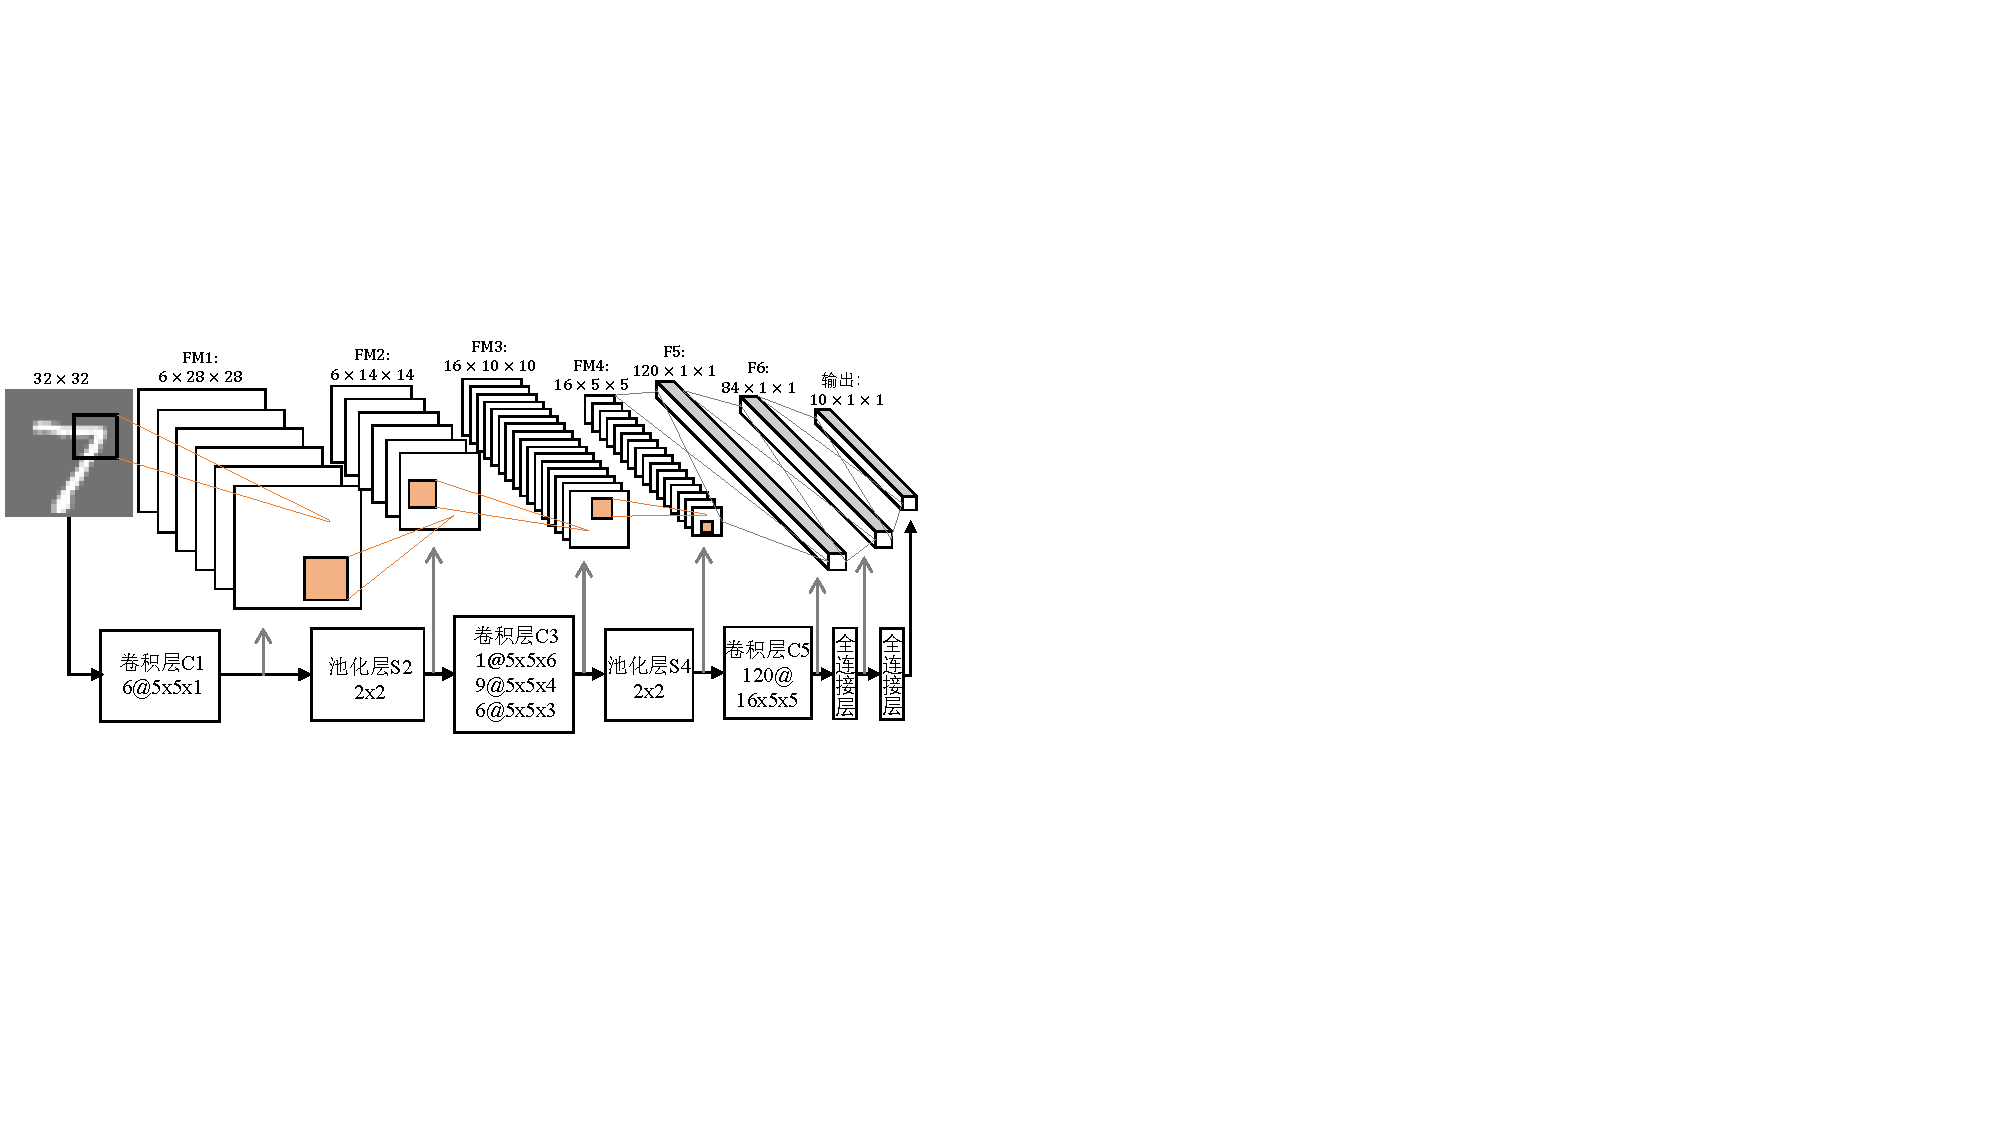
\includegraphics[scale=0.9]{Img/fig_2_lenet5.pdf}
    \bicaption{LeNet-5模型示意图}{Schematic diagram of the LeNet-5 model}
    \label{fig:2_lenet5}
\end{figure}
LeNet-5是最早的卷积神经网络模型之一,设计之初被用于手写数字识别任务。图\ref{fig:2_lenet5}展示了LeNet-5从输入图片到输出预测结果的模型工作简化图。LeNet-5共包含5层,包括两个卷积层(convolutional layer)C1、C3、C5,以及两个池化层(pooling layer)S2和S4。

{\sffamily 卷积层:}卷积层是CNN模型的核心模块,包含了整个模型的大部分参数。它可以对输入图像的局部区域进行加权求和从而得到图片的特征(feature)或特征图(feature map,FM),例如示例中经过卷积层得到的特征或特征图有FM1、FM3和F5。卷积层中卷积核(convolution kernel)大小和形状的选择能够影响卷积的效果。例如,图\ref{fig:2_lenet5}中卷积层C1中有6个$5 \times 5 \times 1$的卷积核,每个卷积核将图片中每个$5 \times 5$大小区域内的像素点加权求和得到输出特征图中的一个像素点,因此一个$32 \times 32$大小的图片经过卷积层C1后得到的特征图FM1的大小为$6 \times 28 \times 28$。经过卷积层后,图片的通道数可能会增加,图片的尺寸也可能变小。卷积层的设计可以很简单也可以非常的复杂,例如卷积层C3中包含了16个卷积核,其中各卷积核的尺寸为$5 \times 5$,但选取的特征图数量(图中包含6,4,3三种数量的差别)却各不相同。这说明卷积层的设计可以是非常灵活的,也因此对模型设计与研究人员的考验也是巨大的。

{\sffamily 池化层:}池化层一般也称为下采样层(subsampling layer),相当于一个过滤器,对图片或特征图执行降维操作,滤掉无用的像素点,帮助模型提取更高层次的特征。其原理是在输入特征图中一个局部区域内,按照选取最大值或计算平均值的方式为输出特征图增加一个新的像素点,也称最大池化(max pooling)和平均池化(average pooling)。例如图\ref{fig:2_lenet5}中的池化层S2的大小为$2 \times 2$,它在图片中对应区域内选取最大值或计算平均值后输出到特征图FM2中。区别于卷积层,池化层对输入特征图进行过滤像素时,一般不设置重叠区域,例如图中的池化层的尺寸和步长均为2,因此特征图经过池化层后特征图的尺寸变为原来的二分之一。

{\sffamily 全连接层:}全连接层(full connection layer)层中的每个神经元都连接着上一层的所有神经元。区别于卷积层和池化层将图片映射到隐层的特征空间中,全连接层将隐层表示映射为图片的分布式特征表示,或经过非线性激活函数(一般采用softmax函数)得到样本的概率模型并预测样本的分类结果。例如图\ref{fig:2_lenet5}中最后的全连接层将图片特征F6映射为一个维度为10的向量中,每个维度的取值为0到1,代表着预测为0到9每个值的概率。

虽然LeNet-5的结构简单,但依旧展现了卷积神经网络能够学习并表征图片信息的能力。层数更深,网络结构更复杂,以及采用了更多新技术的新一代卷积神经网络能够表征更复杂的图像信息。在融合视觉信息的自然语言处理任务中,因文本输入与图片输入很难在一个模型中同时支持,因此通常采用特征融合的方式支持多模态输入。从一般的卷积神经网络的模型结构可以看到,选取图片特征的选择可以有很多种。例如图\ref{fig:2_lenet5}中FM4的尺寸为$16 \times 5 \times 5$,其中,在$5 \times 5$的特征图内仍保留着与源图片中的区域对应关系。因此FM4可看作是由$5 \times 5$个维度为16的特征组合而成,每个16维的特征表征了图片中对应的区域。这种保留了图片内局部空间信息的特征图一般称为栅格特征(grid feature)或局部特征(local feature)。在融合图片信息的神经机器翻译方法中,栅格特征一般可以作为图片输入序列输入到翻译模型中,通过注意力机制能够动态地关注到栅格特征中保留的局部空间信息。利用平均池化将栅格特征所代表的多个视觉特征融合为一个视觉特征,称作全局特征(global feature)。全局特征表征了图片的全局信息,通常可以用于初始化循环神经网络,或作为词向量等方式输入到神经机器翻译模型中。

% 要强调栅格信息保留了位置信息
% 这里最好直接举ResNet的例子,可以直接将残差连接的引入到现有机器翻译模型中

\subsection{目标检测方法}
\label{sec:2_object_detection}
%方法背景介绍

\begin{figure}[!htbp]
    \centering
    \begin{subfigure}{\textwidth}
      \centering{
      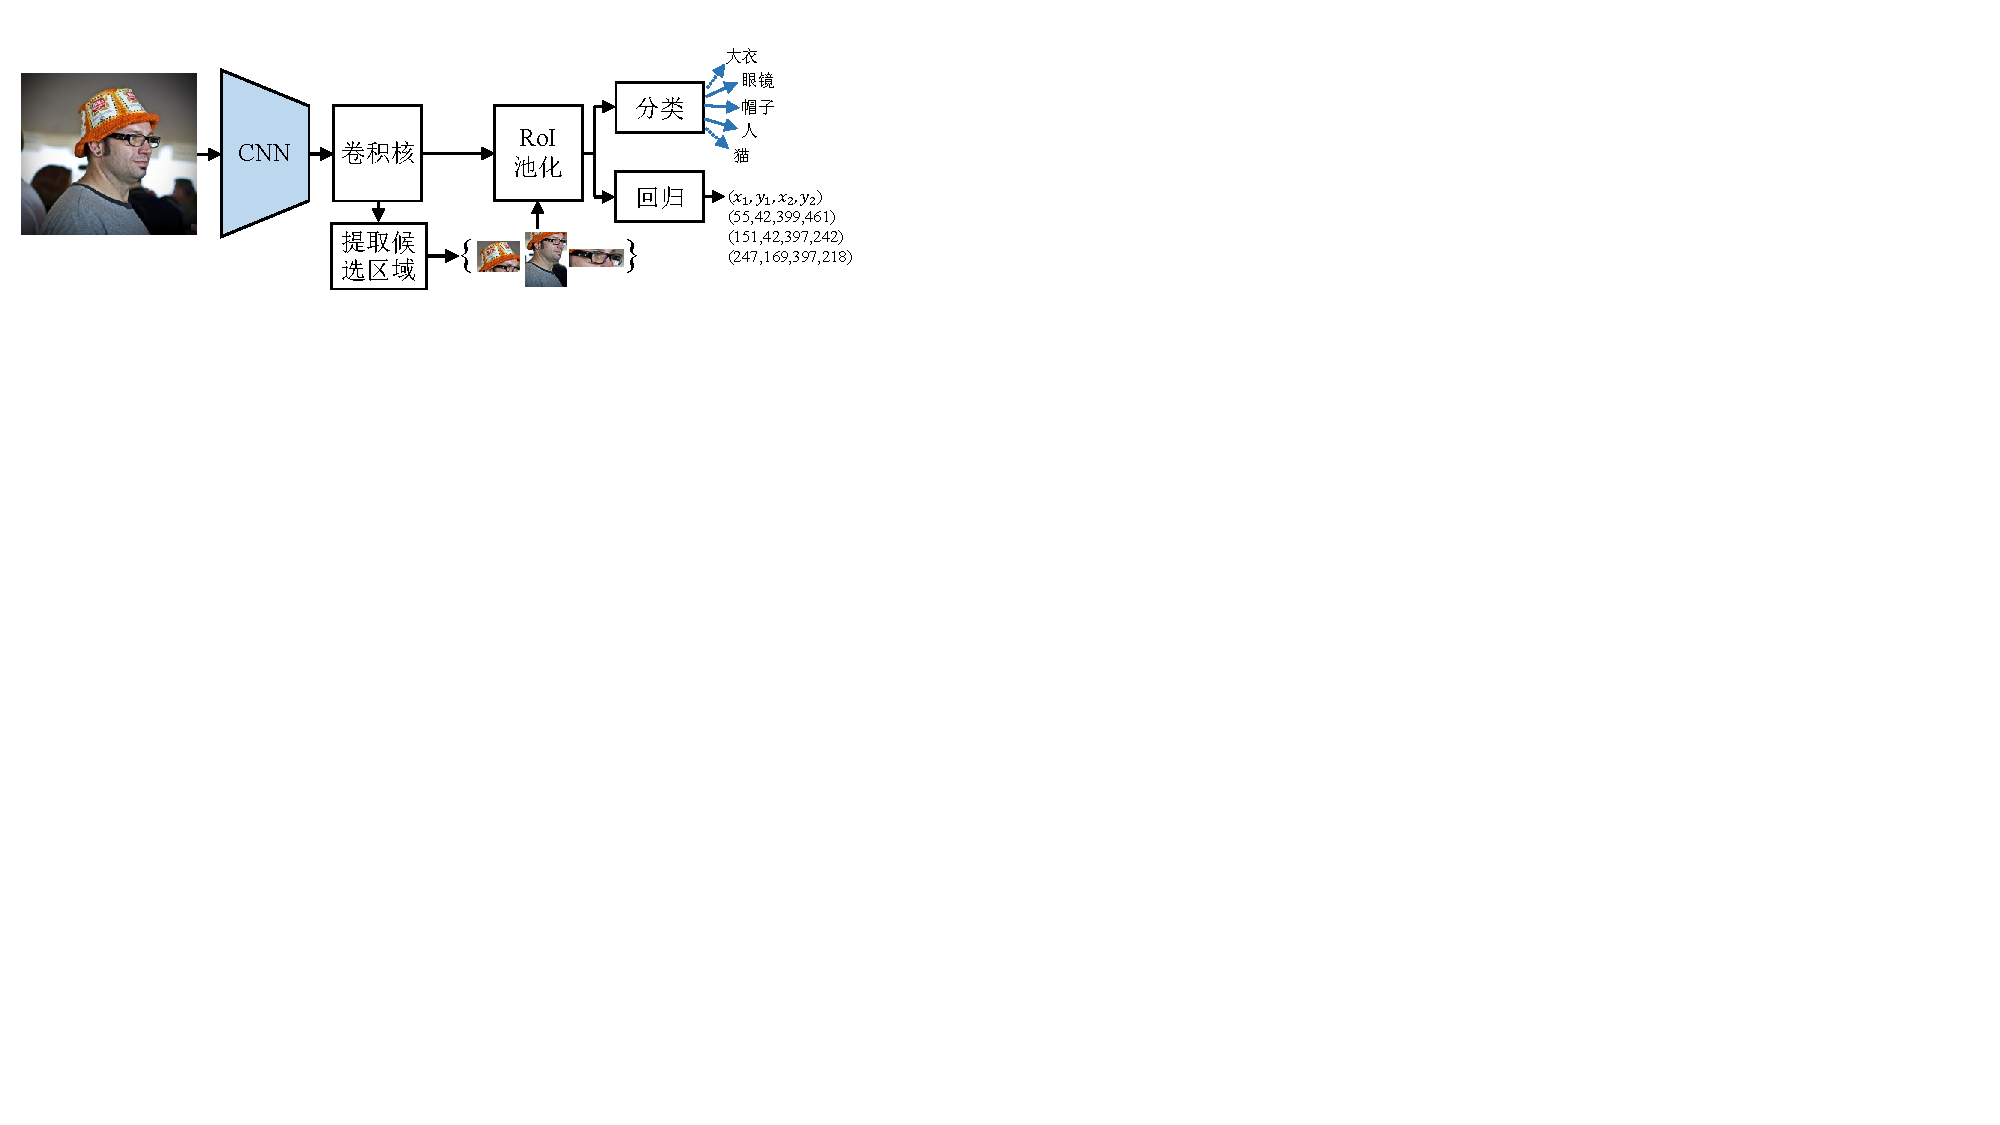
\includegraphics[scale=1.0]{Img/fig_2_rcnn.pdf}
      \caption{两阶段目标检测算法简图}
      \label{fig:2_rcnn}}
    \end{subfigure}%
    \\% line break
    \begin{subfigure}[b]{\textwidth}
      \centering
      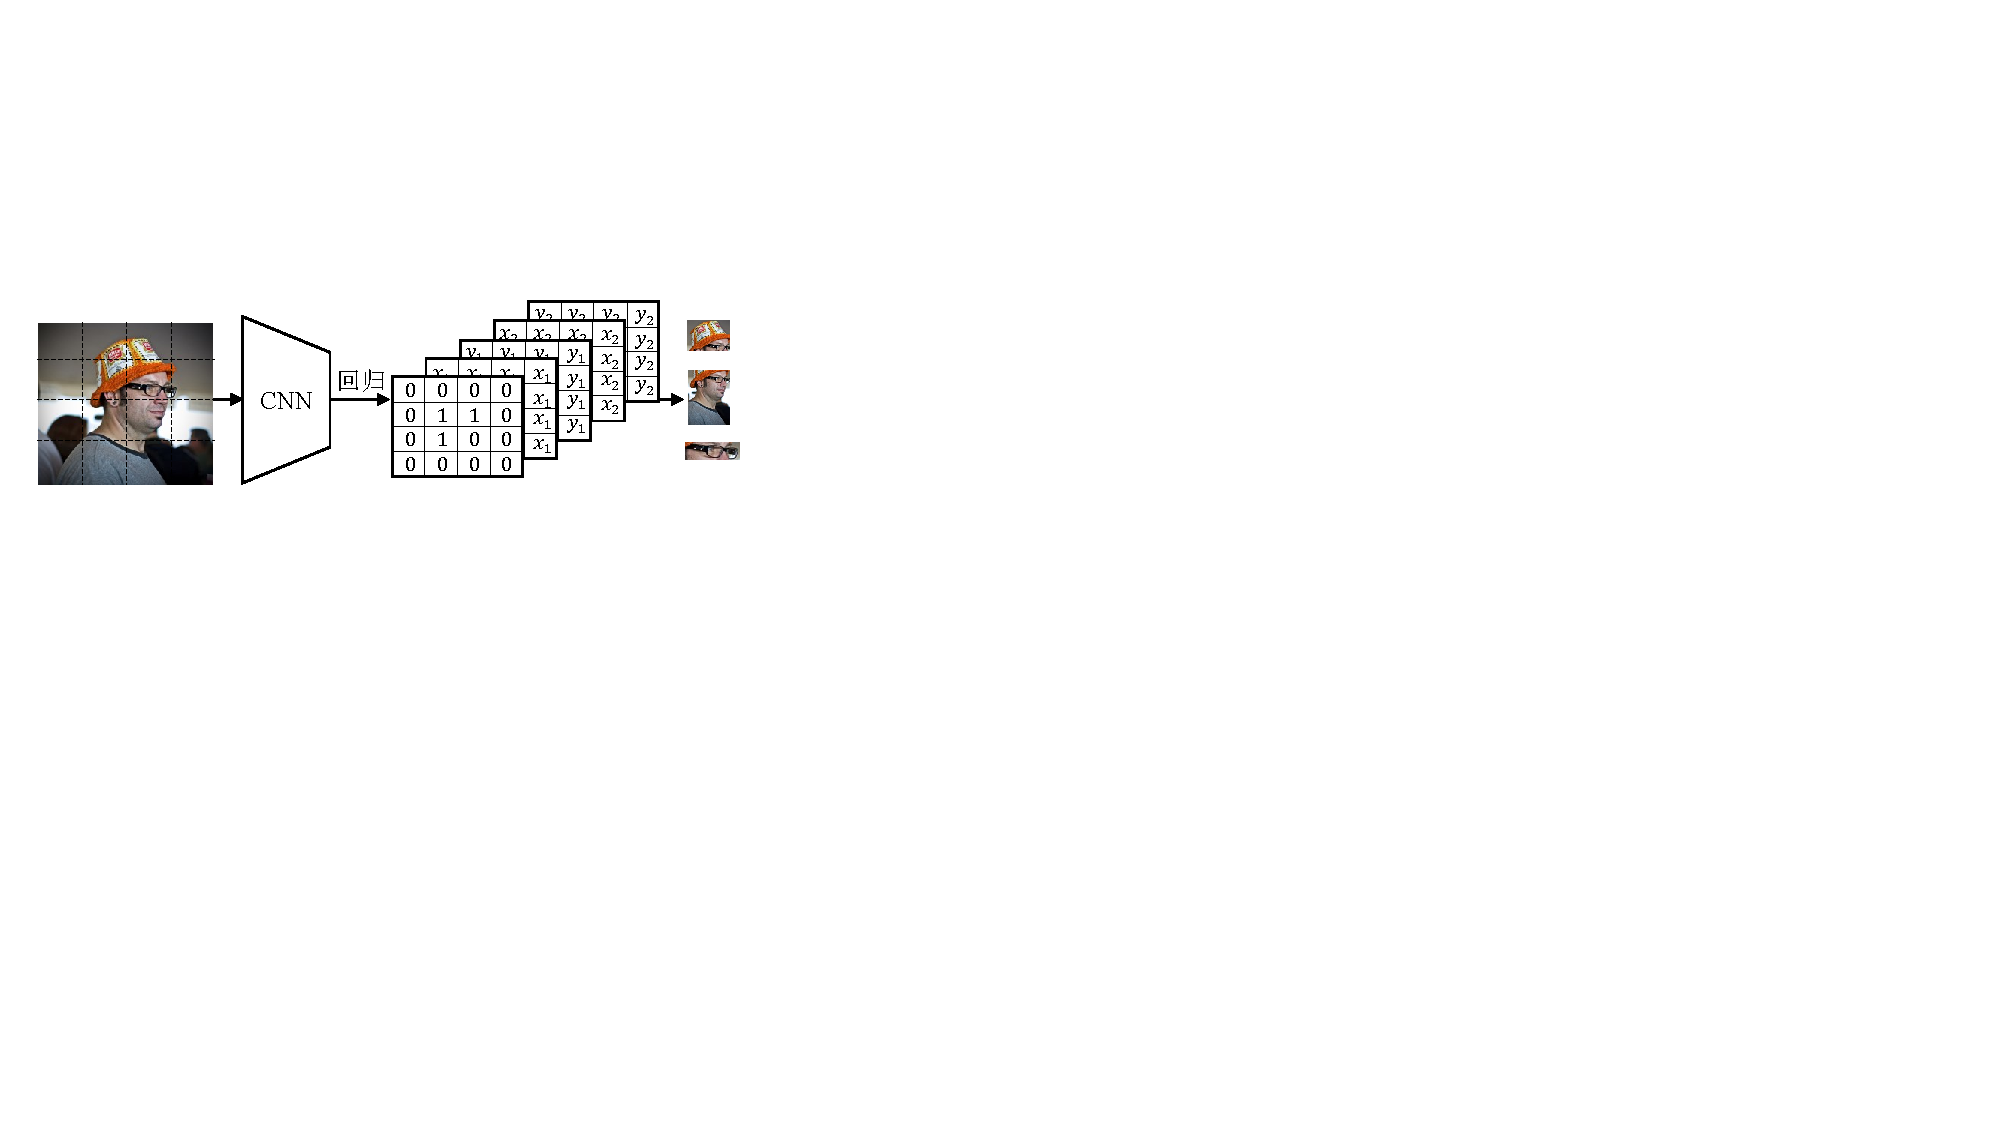
\includegraphics[scale=1.0]{Img/fig_2_yolo.pdf}
      \caption{一阶段目标检测算法简图}
      \label{fig:2_yolo}
    \end{subfigure}
    \\% line break
    \begin{subfigure}[b]{\textwidth}
      \centering
      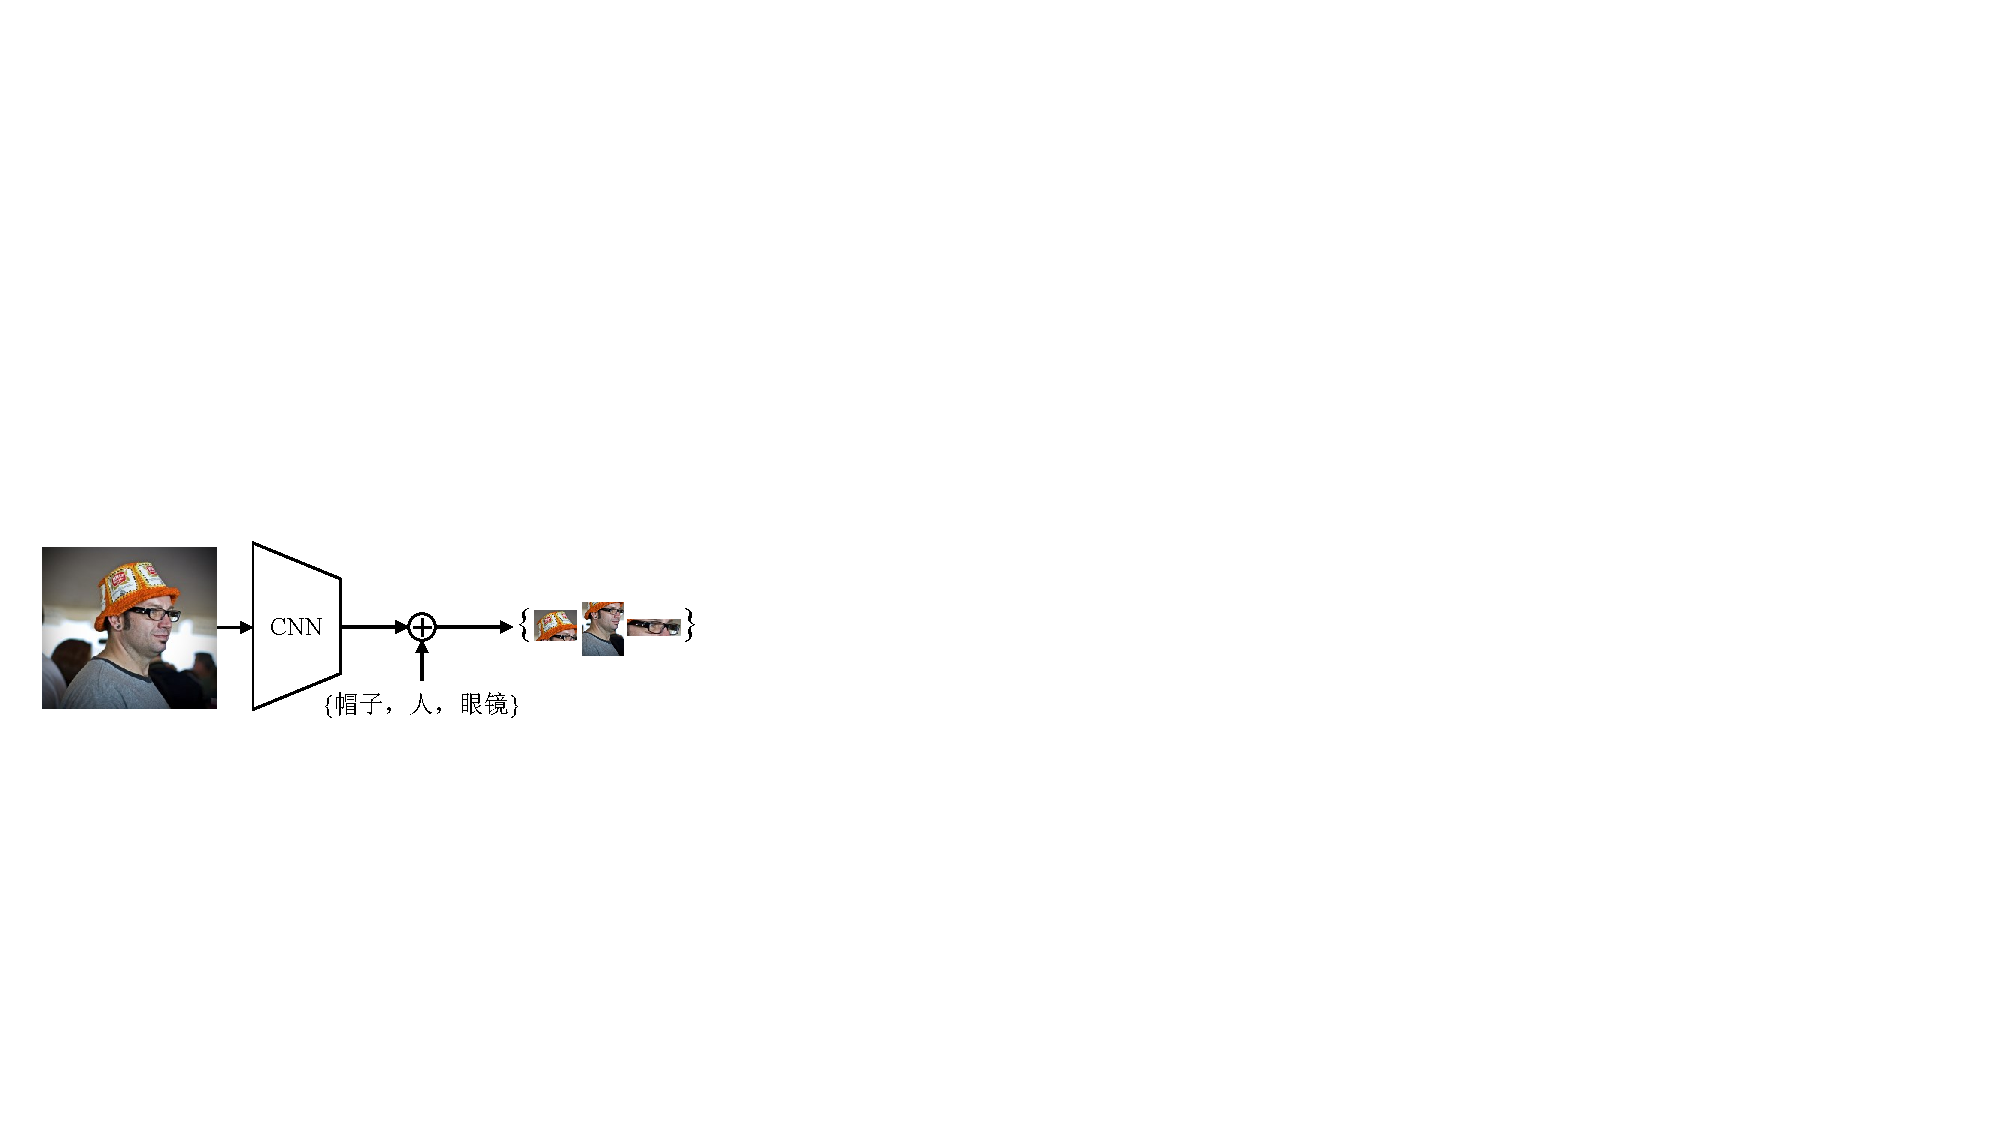
\includegraphics[scale=1.0]{Img/fig_2_visual_grounding.pdf}
      \caption{语义目标提取法简图}
      \label{fig:2_visual_grounding}
    \end{subfigure}%
    \bicaption{目标检测算法示意图}{Schematic diagram of object detection algorithm}
    \label{fig:2_object_detection}
\end{figure}
目标检测是计算机视觉领域中一个应用范围非常广的任务,其目的是在图像或视频中自动地定位并识别出特定的视觉目标,从而满足对视觉目标的筛选、分类、追踪等需求。早期的目标检测算法需要手工设计特征和分类器来实现物体检测,并且运行速度较慢。随着深度学习的发展,目标检测算法开始采用卷积神经网络作为基础模型实现对视觉目标的检测,并取得了很好的性能与速度。对于融合图片信息的神经机器翻译任务,目标检测同样是非常重要的应用手段之一。与卷积神经网络能够提供图片的全局特征和栅格特征相比,目标检测的结果能够直接将图片中最有价值的前景信息提供给翻译模型。并且,每个视觉目标都能够提供排除与视觉目标不相关的更集中的视觉信息。

根据各算法特点以及工作方式,可以将目前常用的目标检测算法可以分为三类:两阶段法、一阶段法、语义目标提取法(visual grounding)。其中两阶段法和一阶段法提取给定图片中的所有类别可知的目标,并将提取出的目标分到相应的类别。语义目标提取法是根据语义信息提取相应的视觉目标,因此可以与前两者区分开。

{\sffamily (1)两阶段法}

两阶段法的代表方法有R-CNN(region-based convolutional neural networks)\pcite{girshick2014rich}、Fast R-CNN\pcite{girshick2015fast}以及Faster R-CNN\pcite{ren2015faster},如图\ref{fig:2_object_detection}(a)。这类算法在目标检测过程中通常分为提取候选区域(region proposal)和特征提取与分类回归两个阶段。
从图片中提取视觉目标的最简单方式就是采用滑动窗口方法遍历图片中所有的矩形区域,然后利用分类器将有效的矩形区域分类到与其对应的类别。很显然,这种枚举的做法会消耗大量的检测时间。因此常见的两阶段法都会采用精心设计的算法提取出图片中的部分候选区域。
例如,在R-CNN中采取了选择性搜索(selective search)算法在原始图片中提取出1000至2000个候选区域,也称感兴趣区域(region of interest,RoI),这种做法的弊端就是需要对这些候选区域都进行一次CNN的编码,同样耗费很多时间。
而Fast RC-NN为了节省这部分时间先将图片经过CNN表征后再利用其所设计的RoI池化方法将栅格特征中与RoI相对应的区域提取出来。
为了更进一步地提高效率,Faster R-CNN方法采用了区域提取网络(region proposal network,RPN)代替耗时的选择性搜索算法。
通过第一阶段的提取就可以得到每个RoI的特征表示了。采用深度学习算法之前都是通过人工设计的特征来表征图片,而目前都是通过CNN来更方便的表征图像信息。将RoI的特征表示经过分类器就可以判断当前RoI是否属于某个已知的类别从而完成对提取到的视觉目标的分类。同时还要经过回归算法来获得目标的更精确的方框定位(bounding box)。

{\sffamily (2)一阶段法}

一阶段法的代表方法为YOLO(you only look once)\pcite{redmon2016you,redmon2017yolo9000,redmon2018yolov3,bochkovskiy2020yolov4,ge2021yolox}系列算法,其特点是采用单个神经网络同时完成对图像中视觉目标的提取和分类,而不需要预先生成候选区域。因此,一阶段法具有更快的目标检测速度。图\ref{fig:2_object_detection}(b)展示了YOLO算法的简化示意图,其基本工作原理是直接采用回归的方式替代预提取和分类的组合方式,利用CNN对图像的表征对图片中的方框坐标$(c,x_1,y_1,x_2,y_2)$进行回归,从而达到仅需要进行一次CNN的前向计算就能够得到检测结果的目的,其中$c$代表预测的置信度(confidence),$(x_1,y_1)$与$(x_2,y_2)$分别代表方框的左上角和右下角在图片中的位置坐标。为了能够一次提取图片中的多个视觉目标,则将输入图片划分为多个区域,每个区域负责一个视觉目标的提取。当视觉目标的中心落在某个区域时,该区域负责对该视觉目标的提取,例如图\ref{fig:2_object_detection}(b)中,图片被虚线分割的每个矩形区域与矩阵中每个位置一一对应,矩阵中“1”的位置分别对应了图片中“人”、“帽子”和“眼镜”的中心所在的矩形区域。

{\sffamily (3)语义目标提取法}

在图片中提取与文本语义相关区域的方法是语义目标提取法,方法示意图如图\ref{fig:2_object_detection}(c)所示。这类方法的输入是一张完整的图片和需要提取内容的文本。例如提取图片中的“人”时,其模型输入为图片和文本“人”、“男人”或者“一个戴眼镜的男人”。提取视觉目标的过程需要对图片和文本先编码,然后利用跨模态信息融合的方式识别出图片中与文本语义最相近的区域。最初的语义目标提取可以认为是目标检测任务的下游任务,所用的方法是先采用常用的目标检测方法将图中的视觉目标提取出来并分类。然后根据视觉目标类别与输入文本相似度通过匹配的方式完成语义目标的提取。这种传统的语义目标提取方法因为需要两种方法相结合才能完成任务,因此也称为两阶段法。而图\ref{fig:2_object_detection}(c)中所展示的方法不需要先提取再匹配的过程,所有提取步骤在一个统一的模型中完成,因此称为一阶段法。采用语义目标提取法获得视觉目标的方式能够将文本的内容与图片中的视觉目标对应起来,对于跨模态信息融合有很大的帮助。本文在后面的章节\ref{sec:3_entity_extraction}小节所介绍的工作就采用了一种一阶段的语义目标提取法,来获取句子中的短语与图片中的视觉目标的对应关系。
%方法介绍

%在ImgNMT中的应用

%对于跨模态信息融合,目标检测依旧是非常重要的应用手段之一。与卷积神经网络相比,目标检测的结果能够直接将图片中那些信息量最大的目标直接提供给翻译模型,而提取出的视觉目标所包含的信息也更集中。目标检测的结果可以分为两种,一种是检测结果与文本不建立关系,此时目标检测方法输出的多个视觉目标结果可以视为视觉目标序列输入到以序列建模擅长的自然语言处理任务的模型中。另一种是通过文本语义进行视觉目标检测,这种方式能够对齐文本与视觉目标,更方便在翻译中使用。
% 目标检测要给出区域,和分类
% 最初的设定,扫描图片中的所有框
% R-CNN:two-stage,ROI->feature extraction for ROI->SVM->位置精修
%      R-CNN-> Fast R-CNN -> Faster R-CNN
% Yolo v0-5: one-stage (you only look once)(regression)
%      v0: 遍历所有“框” -》 输出(c,x,y,w,h) 其中c为confidence,label为(1,x*,y*,w*,h*)
%      v1:检测多个目标,将img划分为多个区域,(c,x,y,w,h,one-hot)*N
% visual grounding

%\subsection{视觉Transformer}
%这里和前面呼应以下,前面是CV推动着NLP的发展,这里则反过来,NLP推动CV

%预示着大模型的融合

%与CNN相同同样可以做backbone,做目标检测以及图片分类

% 结尾说以下那几篇文章说过使用哪种CNN-backbone带来的差别并不大
% 2.4 MMT
\section{融合图片信息的神经机器翻译}
\label{sec:2_imgnmt}

%研究意义与背景介绍
得益于深度学习技术在自然语言理解和计算机视觉等领域的快速发展,融合文本与图片信息的跨模态理解与生成也成为了可能。融合图片信息的神经机器翻译就是将已经成熟的计算机视觉方法与神经机器翻译技术相结合的一类研究。其研究历程也紧随着纯文本神经机器翻译的脚步而发展。一个标准的神经机器翻译系统通常以句子为翻译单位。端到端的翻译模型通过拟合大量双语数据中语言之间的对齐特性习得翻译能力,在编码过程将源语言句子的信息编码为分布式的向量表示,再通过解码器将表示向量解码到目标语言。然而,针对翻译采集的数据也包含着人类语言应用中的使用习惯与问题。例如文本中存在多译词、歧义词或者不完整表达等问题,都需要通过待翻译句子以外的补充信息来解决,而图片中往往包含着更丰富、更完整以及更准确的信息。因此在翻译一个句子时,图片中的视觉信息能够其提供所需的外源补充信息。为此,研究者们提出了融合图片信息的神经机器翻译方法(image-incorporated neural machine translation,ImgNMT)。

% 任务定义
融合图片信息的神经机器翻译方法的目的是在基于神经机器翻译的框架内,借助图片信息生成更准确译文。该方法是多模态机器翻译(multi-modal machine translation)的一个研究子类。相关的多模态机器翻译还包含口语翻译\cite{82_DBLP:conf/icassp/Vidal97,83_DBLP:conf/icassp/Ney99,84_DBLP:conf/interspeech/WeissCJWC17,85_DBLP:conf/icassp/BerardBKP18}(spoken language translation,SLT)和视频引导翻译\cite{86_DBLP:conf/lrec/LisonT16,87_DBLP:journals/corr/abs-1811-00347,88_DBLP:conf/iccv/WangWCLWW19}(video-guided translation,VGT)\cite{81_DBLP:journals/mt/SulubacakCGREST20}。目前已知的多模态翻译方法多数是融合了两个模态信息的跨模态方法。视频引导翻译与融合图片信息的翻译任务有着相似的特点,都是在文本翻译的基础上通过融合视觉信息提升翻译性能,但也因此相关研究较少。

% 研究方法及其分类
作为多模态机器翻译领域的一个重要方向,ImgNMT得到了学界的广泛关注。2016年机器翻译研讨会(workshop on machine translation,WMT)开展多模态机器翻译的相关评测\cite{112_specia-etal-2016-shared},彼时的多模态机器翻译任务的目标是为图片生成目标语言的译文,因此可分为两种解决方案:第一种是利用图片信息生成目标语言句子,这种任务形式一般称为图像描述生成(image captioning)或图像翻译;另一种就是在文本翻译任务中加入图片信息辅助翻译过程,也就是本文关注的ImgNMT。在此之后,WMT 2017\cite{113_elliott-etal-2017-findings}和WMT 2018\cite{114_barrault-etal-2018-findings}将多模态机器翻译的研究进一步推向全世界,越来越多的相关研究相继涌现。本节对融合图片信息的神经机器翻译的国内外研究现状进行了系统的梳理和分类。本文将相关研究分为四个类别:图片信息辅助式神经机器翻译、图片信息增强式神经机器翻译、基于图片搜索的神经机器翻译以及跨模态无监督神经机器翻译,并分别在后续的小节中进行详细的介绍。

%得益于神经网络方法的快速发展,自然语言文本与图片的信息融合成为了可能。融入图片信息的机器翻译的研究历程也紧随着纯文本的神经机器翻译的脚步而发展。然而,相关研究则最早起源于图像描述生成任务。有部分学者将文本作为一个外源信息来辅助图片描述的生成,但这种方式的本质则是在翻译任务中融入视觉信息。2016年WMT将多模态机器翻译引入作为共享任务后,MMT受到了广泛的关注。在之后的WMT17和WMT18,MMT任务延续并奠定了在机器翻译中融合图片信息作为多模态机器翻译研究的主要范式。

%平行翻译句一般具有良好的对齐特性,这使得融入的外源信息仅用于辅助少数具有歧义、信息不完整以及训练不充分等问题的句子的翻译。该特性也成为了展开相关研究道路上的一大难点。
%融合图片信息的神经机器翻译任务主要采用的是平行翻译句对加图片三元组形式的数据,即一张图片对应一句描述和一句翻译。大部分相关研究需要对神经机器翻译模型进行适当的修改,以适应图片的输入。模型中输入的图片可用于辅助优化翻译过程中源语言的语义表示,或为解码过程增加辅助外源信息。本文将这种在翻译过程中以源端文本作为信息主体,输入图片用于语义信息强化的方法称为图片信息辅助式神经机器翻译。可根据图片信息融合到翻译模型中的方式将这种方法分为三类:融合图片全局信息、融合图片局部动态信息以及融合图片视觉目标信息。这些三种图片信息以视觉特征为载体输入到翻译模型中,视觉特征则是从预训练的卷积神经网络中提取得到。不同的提取方式所包含的语义信息的粒度和特征维度有所不同。将这些不同形式的视觉特征整合到NMT模型后,模型进行跨模态语义融合的难易程度则取决于模型设计的合理性。


%以下两种方式合并讨论:
% 还可分为编码融合方法,和解码融合方法
% 全局 局部 视觉目标

% 显式、隐式:放到最后与igt和iet交叉讨论
% 这个章节中可以多提一下ImgNMT与多模态摘要任务的区别
\subsection{图片信息辅助式神经机器翻译}
\label{sec:2_ignmt}
\begin{figure}[!htbp]
    \centering
    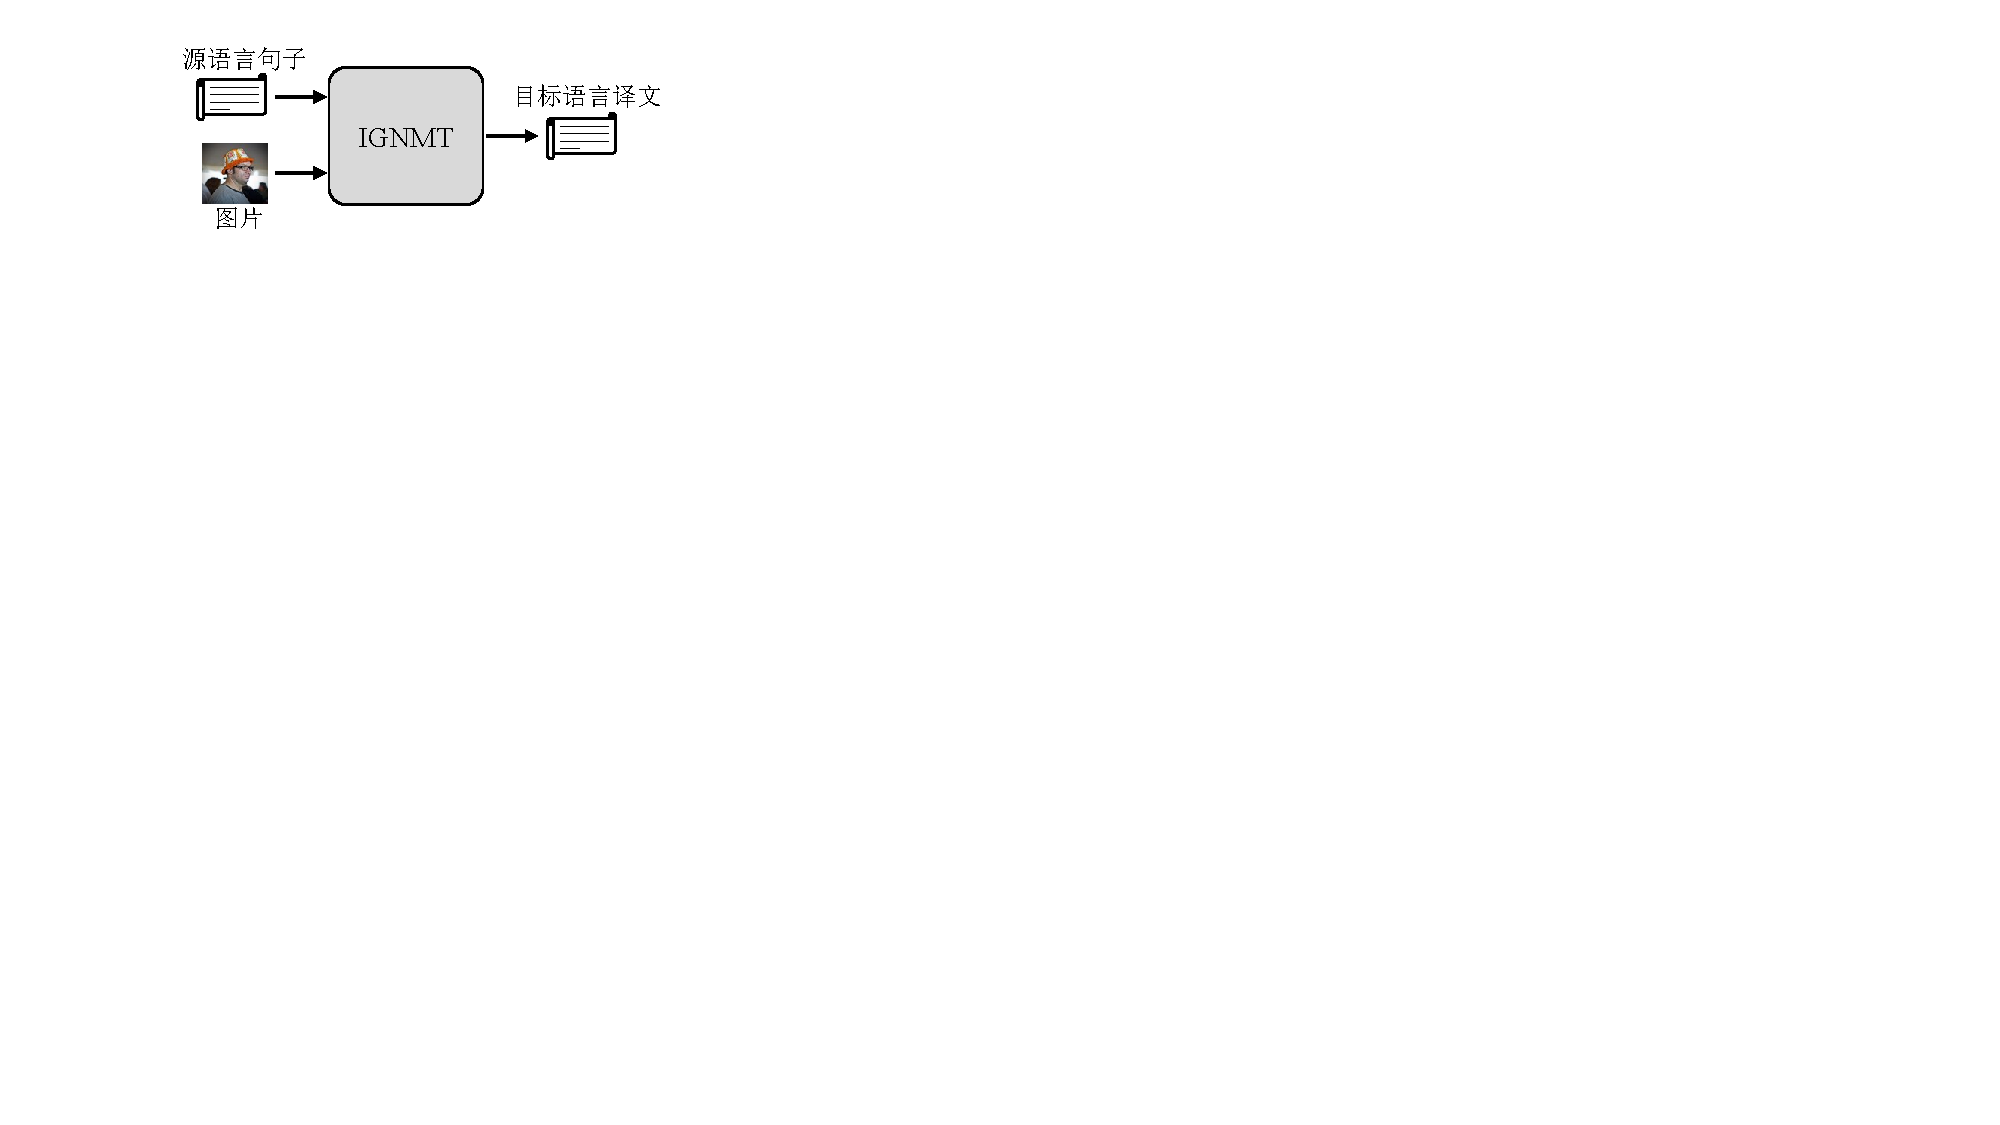
\includegraphics[scale=1]{Img/fig_2_ignmt.pdf}
    \bicaption{图片信息辅助式神经机器翻译}{Image-guided neural machine translation}
    \label{fig:2_ignmt}
\end{figure}
图片信息辅助式神经机器翻译方法又称图片引导式神经机器翻译方法(image-guided neural machine translation,IGNMT),是融合图片信息的神经机器翻译方法中最常见的一类分支,也是融合图片信息最自然的一类方法,理论上还是视觉信息利用程度最高的一类方法。这类方法的特点是将图片直接输入到翻译模型中,通过直接的模型学习或某种人为设计的方式,使翻译模型在进行编码源语言句子或解码目标语言句子时,通过利用输入的图片信息完成更好的编码表示或进行更准确的解码生成,从而得到更准确的译文。因采用编码器-解码器结构的翻译模型具有非常灵活的使用方式,同时在\ref{sec:2_cv}节中提到,图片特征的提取方式也分为多种,所以将图片信息融合到翻译模型中的方法也有很多。本节将这些方法从两个方面进行分类,从作用到翻译模型结构中的不同组成部分可分为:编码融合方式和解码融合方式;从图片的视觉特征使用方式的不同可分为:全局特征融合方法、局部特征融合方法以及视觉目标特征融合方法。

\subsubsection{基于模型结构的图片信息融合方法}

{\sffamily (1)编码融合}

基于编码器-解码器结构的神经翻译模型中,编码器负责将源语言句子编码为向量表示。在编码前,源语言句子中的单词会被转换成利用分布式向量表示的词向量。在编码过程中,分散在输入序列的信息将通过循环神经网络或多头自注意力机制按照序列内各项的位置信息交织并融合,序列中每一项的特征向量不再是一个单独的表示,而代表着融合了句子中上下文信息的向量表示。在编码后,句子的隐层向量表示将传递给解码器用于解码目标语言。在编码的前、中、后三个阶段,均是图片信息可以参与的阶段。

\tcite{calixto2017incorporating}尝试在编码前,将图片的全局特征以前、后以及两侧三种方式与源语言句子词向量序列拼接,然后将图片信息融合到源语言句子的编码中。\tcite{huang2016attention}提出了另外两种方案,一是利用R-CNN提取出图片中视觉目标的全局特征,然后连同完整图片的全局特征作为序列拼接到文本输入前,最后利用编码器一起编码;二是将每个视觉目标单独拼接到文本序列前,然后对每个这样的序列都进行一次单独的编码,在解码的过程中需要通过注意力机制选择与当前解码状态最相关的那个编码序列。为了使模型更充分地学习跨模态信息的融合,还可以采用大规模视觉语言预训练模型(vision-language pre-trained model)的方案\pcite{caglayan2021crosslingual,wang2021make,susanto2021rakutens,yawei2021probing,hirasawa2022pretrained}。这种方法主要利用更大规模的数据和更多模型参数的优势使模型具备更强的跨模态信息融合能力,其模型多是基于Transformer结构,模型的输入是句子和图片的组合方式。不难看出,虽然各类方法在编码前阶段就需要将图片与文本拼接到一起,但该过程并不能起到信息的融合作用,仅影响了图片在模型编码过程中的作用方式。这些方法的跨模态信息融合过程依赖的是循环神经网络或基于自注意力机制的Transformer编码器所具备的序列建模能力。

在编码前将图片和句子组合的方式具有方法简单的优点,但通常也会增加模型的学习难度。因此,有相关工作尝试利用模型或数据的特点,通过设计模型的使用方式或模型结构,使模型在编码的过程中融合图片信息。最早的相关工作利用图片的全局特征初始化基于循环神经网络的编码器的初始状态\pcite{elliott2015multilanguage,calixto2017doubly}。\tcite{yang2020visual}在编码的过程中通过建立视觉目标特征序列和文本表示序列的相似度矩阵,得到文本序列与视觉目标序列之间的相似度,并在进一步的文本表示编码中将相似度作为注意力值加权计算,最后为了提升图片信息的作用,在训练过程中加入了正则化损失。\tcite{yin2020novel}采用了图结构建模源语言句子与图片中视觉目标的关系,然后设计了基于多头注意力机制的面向图结构的多模态编码器,在编码的过程中将视觉目标节点和文本单词的节点单独编码,然后再用交叉注意力机制获得单词节点的视觉目标特征表示和视觉目标特征的单词表示,最后将文本节点的编码结果传递给一个常规的解码器。

在翻译的编码过程完成后再进行视觉信息融合的方法相当于利用图片对文本表示进行二次编码。\tcite{wang2021efficient}在文本编码器得到隐层表示后,增加了视觉目标与源语言句子之间的关联表示。该方法设计了以多头注意力为基础的目标-源注意力层(object-source attention layer),建立文本序列的视觉目标表示,并在损失函数中加入了目标掩码损失函数使模型更多的关注与源语言信息相关的视觉目标。\tcite{wu2021good}和\tcite{li2021vision}都在编码后采用了门控机制,利用图片的全局特征与文本向量表示语义关系,建立能够控制图片全局特征编码参与度的门控向量,最后将门控向量作用到文本的隐层向量与图片全局特征的加权和上。

{\sffamily (2)解码融合}

基于编码器-解码器结构的神经翻译模型中,解码器负责将编码过的文本向量表示解码到目标语言。而该过程是自回归解码(autoregressive decoding),即解码目标语言句子时每个时间步只能生成一个单词,每个单词的生成需要依赖前面的解码时间步和源语言所提供的信息。源语言提供了整个句子的完整的静态信息,前面时间步已经解码的结果为解码器提供当前时间步需要哪些动态信息。从解码器的工作方式不难看出,图片在解码过程中的主要作用与源语言句子类似,提供的是静态信息。
与编码器类似,早期方法将图片的全局特征作为完整的视觉语义信息用于初始化基于循环神经网络的解码器的初始状态,从而在解码的循环迭代中,在隐层向量中保留着图片所提供的信息\pcite{elliott2015multilanguage,calixto2017incorporating,zhou2018visual,zheng2018ensemble}。

然而,这种利用图片特征初始化循环神经网络的方式在解码过程中存在遗忘的问题。在解码到后面的单词时,隐层表示中所保留的视觉信息将越来越少,因此这种视觉信息作用方式的效果很有限。除此之外,这种方法仅适用于基于循环神经网络的方法,无法适用于更广泛应用的基于Transformer的神经机器翻译。注意力机制在出现后成为解决这类问题最受欢迎的解决方案。
早期基于循环神经网络的神经机器翻译模型采用了增加图片注意力模块的方式\pcite{caglayan2016multimodal,calixto2017doubly,caglayan2018liumcvc,gain2021iitp,laskar2021improved}。图片注意力模块的实际工作方式与文本注意力模块是相似的,可以根据当前解码状态判断图片的栅格特征中哪些区域的视觉信息对于解码当前步的单词是有用的。因此这种方法能够为解码器提供动态的图片局部信息。
\tcite{zhao2020double,zhao2021tmeku}同样采用了双注意力机制的方案,不同的是,该方法提供的是从Faster R-CNN中提取的视觉目标序列。
在基于Transformer的神经机器翻译模型的解码器中,一般采用的是增加针对图片的交叉注意力模块\pcite{arslan2018doubly,gronroos2018memad,libovicky2018input}。
\tcite{liu2021gumbel}认为这些方法很难使模型注意到图片中的有用信息,并且会引入大量的噪音,因此使用了Gumbel-Softmax改造了注意力机制。
\tcite{li2022vision}所提方法并没有采用从卷积神经网络提取出来的图片特征,而是采用了ViT(vision Transformer)\pcite{liu2021swin}模型提取出来的图片特征,然后利用交叉注意力机制和门控机制的组合方式,为解码器提供图片信息。
注意力机制不仅可以在解码过程中使用,同样可以应用于解码后。\tcite{ive2019distilling}在解码器后端增加了用于二次解码的推敲网络(deliberation network),同样使用了注意力机制,并且可以关注源语言信息、视觉目标信息以及第一次的解码信息。

\subsubsection{基于图片特征结构的图片信息融合方法}
在前面的\ref{sec:2_cv}节中介绍到,直接从卷积神经网络中可以提取到全局特征和栅格特征。利用目标检测方法可以提取出图片中最具有前景信息价值的视觉目标。本节,我们根据这些图片特征的特点,对现有的融合图片信息的神经机器翻译方法进行分类。

{\sffamily (1)图片栅格特征}

图片栅格特征一般提取自卷神经网络全连接层之前的输出,例如\tcite{calixto2017doubly}所提方法采用的就是ResNet-50\pcite{he2016deep}全连接层之前非线性激活层的输出。在连入全连接层之前,卷积神经网络对图片进行编码的过程一直保留着图片的二维信息,例如一个大小为$224 \times 224$的图片经过ResNet-50编码得到一个$7 \times 7 \times 2048$的特征表示。其中$7 \times 7$的矩阵将原图片分为49个区域并一一对应,因此这个特征表示可以看做是对图片中49个区域的编码,每个编码的维度是2048。从这种表示方法不难看出,图片栅格特征可以当作对图片编码后产生的编码序列,这个序列的长度为49。在上一小节中介绍的方法中,多数使用注意力机制的方法都应用了图片的栅格特征,并以图片特征序列的形式输入到翻译模型中。与文本序列不同的是,这种形式的图片输入序列的长度是固定的。虽然栅格特征尽可能地保留了图片中的信息,还可以当做图片序列方便模型的设计,但是也存在着一定缺点。一是栅格特征尽可能保留信息的同时也保存了大量与文本翻译不相关的噪音信息,\tcite{liu2021gumbel}就是在这个原因的基础上设计的Gumbel注意力机制。二是这种图片序列与文本序列最大的不同并不是序列的长度是否固定,而是图片中的内容往往更随意,但文本序列满足一定的语法规律。例如图片中的人物可以出现在图片中的任何位置,或者将图片旋转或倒置都不会改变图片内部的主要信息,但是这种操作会对图片信息在栅格特征中的表征位置带来影响\pcite{azulay2019why,kim2020cycnn,mo2022riccnn},最终影响到序列中的位置。这说明了相比于文本序列,图片栅格特征序列所包含信息的位置更随意,使翻译模型难以根据语义信息直接定位到有效信息在栅格特征中的位置。

{\sffamily (2)图片全局特征}

图片全局特征一般来自于将图片的栅格特征经过平均池化层得到的单个表征向量,也可以选择卷积神经网络全连接层的输出向量。例如将ResNet-50的栅格特征经过平均池化后得到一个2048维的图片特征向量,或者像\tcite{calixto2017incorporating}一样采用VGG19\pcite{simonyan2015very}的全连接层输出向量。相比于图片栅格特征,这种全局特征可以看做同样保留了图片完整语义信息。其作用方式与早期基于循环神经网络的神经机器翻译模型用编码器的最后一个隐层向量解码到目标语言类似,同样是利用单个特征向量表征完整的语义。但因为是单个特征向量,所以图片全局特征丢失了图片中的二维空间信息。然而,图片全局特征也有着栅格特征所不具备的优点。一是单个特征的方式更容易嵌入到神经机器翻译模型中,甚至不需要对翻译模型做改动,例如,可以作为词向量或用于初始化模型。二是可以避免卷积神经网络不具备旋转不变性(rotation invariance)带来的问题。

{\sffamily (3)视觉目标特征}

视觉目标特征的提取一般采用目标检测方法提取到视觉目标后,再使用卷积神经网络提取视觉目标的全局特征,或者直接使用目标检测方法自带的卷积神经网络在检测过程中输出视觉目标的全局特征。在使用的数据已有视觉目标的标注情况下,也可以直接将图片中的视觉目标区域裁剪出来,再提取其全局特征。采用视觉目标特征时,通常不使用视觉目标的栅格特征。这是因为视觉目标的信息比完整图片所包含的信息更集中也更明确,并且一般集中于图片中的单个目标。所以多数情况下没有必要保留视觉目标的二维空间信息。视觉目标特征的优点就是在目标提取过程中为每个目标过滤掉了背景信息,使所采用的视觉信息更集中于图片中的关键信息。并且,一张图一般可以提取出多个视觉目标,这些视觉目标可以以排成序列的形式输送给翻译模型。视觉目标特征同样存在着缺点。一是目前的目标检测算法的检测结果与真实的目标区域仍存在着一定的偏差,提取的视觉目标可能并不准确,或仍保留大量的噪音。二是虽然这种方式能够过滤掉背景信息,但也存在着过滤掉有用信息的可能。为了避免这些问题对神经机器翻译模型造成影响,一般采用输入视觉目标特征的同时,也输入完整图片的全局特征\pcite{huang2016attention,ive2019distilling,ive2021exploiting,wang2021efficient}。


%得益于神经网络方法的快速发展,自然语言文本与图片的信息融合成为了可能。融入图片信息的机器翻译的研究历程也紧随着纯文本的神经机器翻译的脚步而发展。然而,相关研究则最早起源于图像描述生成任务。有部分学者将文本作为一个外源信息来辅助图片描述的生成,但这种方式的本质则是在翻译任务中融入视觉信息。2016年WMT将多模态机器翻译引入作为共享任务后,MMT受到了广泛的关注。在之后的WMT17和WMT18,MMT任务延续并奠定了在机器翻译中融合图片信息作为多模态机器翻译研究的主要范式。

%平行翻译句一般具有良好的对齐特性,这使得融入的外源信息仅用于辅助少数具有歧义、信息不完整以及训练不充分等问题的句子的翻译。该特性也成为了展开相关研究道路上的一大难点。
%融合图片信息的神经机器翻译任务主要采用的是平行翻译句对加图片三元组形式的数据,即一张图片对应一句描述和一句翻译。大部分相关研究需要对神经机器翻译模型进行适当的修改,以适应图片的输入。模型中输入的图片可用于辅助优化翻译过程中源语言的语义表示,或为解码过程增加辅助外源信息。本文将这种在翻译过程中以源端文本作为信息主体,输入图片用于语义信息强化的方法称为图片信息辅助式神经机器翻译。可根据图片信息融合到翻译模型中的方式将这种方法分为三类:融合图片全局信息、融合图片局部动态信息以及融合图片视觉目标信息。这些三种图片信息以视觉特征为载体输入到翻译模型中,视觉特征则是从预训练的卷积神经网络中提取得到。不同的提取方式所包含的语义信息的粒度和特征维度有所不同。将这些不同形式的视觉特征整合到NMT模型后,模型进行跨模态语义融合的难易程度则取决于模型设计的合理性。

%\subsubsection{融合图片全局信息的神经机器翻译}


%\subsubsection{融合图片局部动态信息的神经机器翻译}

%\subsubsection{融合图片视觉目标信息的神经机器翻译}



\subsection{图片信息增强式神经机器翻译}
% 这类方法特点不是为了解决语料中自带问题,例如歧义词,而是为了解决模型在训练过程中存在的问题,算是两种不同的思路

\begin{figure}[!htbp]
    \centering
    \begin{subfigure}{0.5\textwidth}
      \centering{
      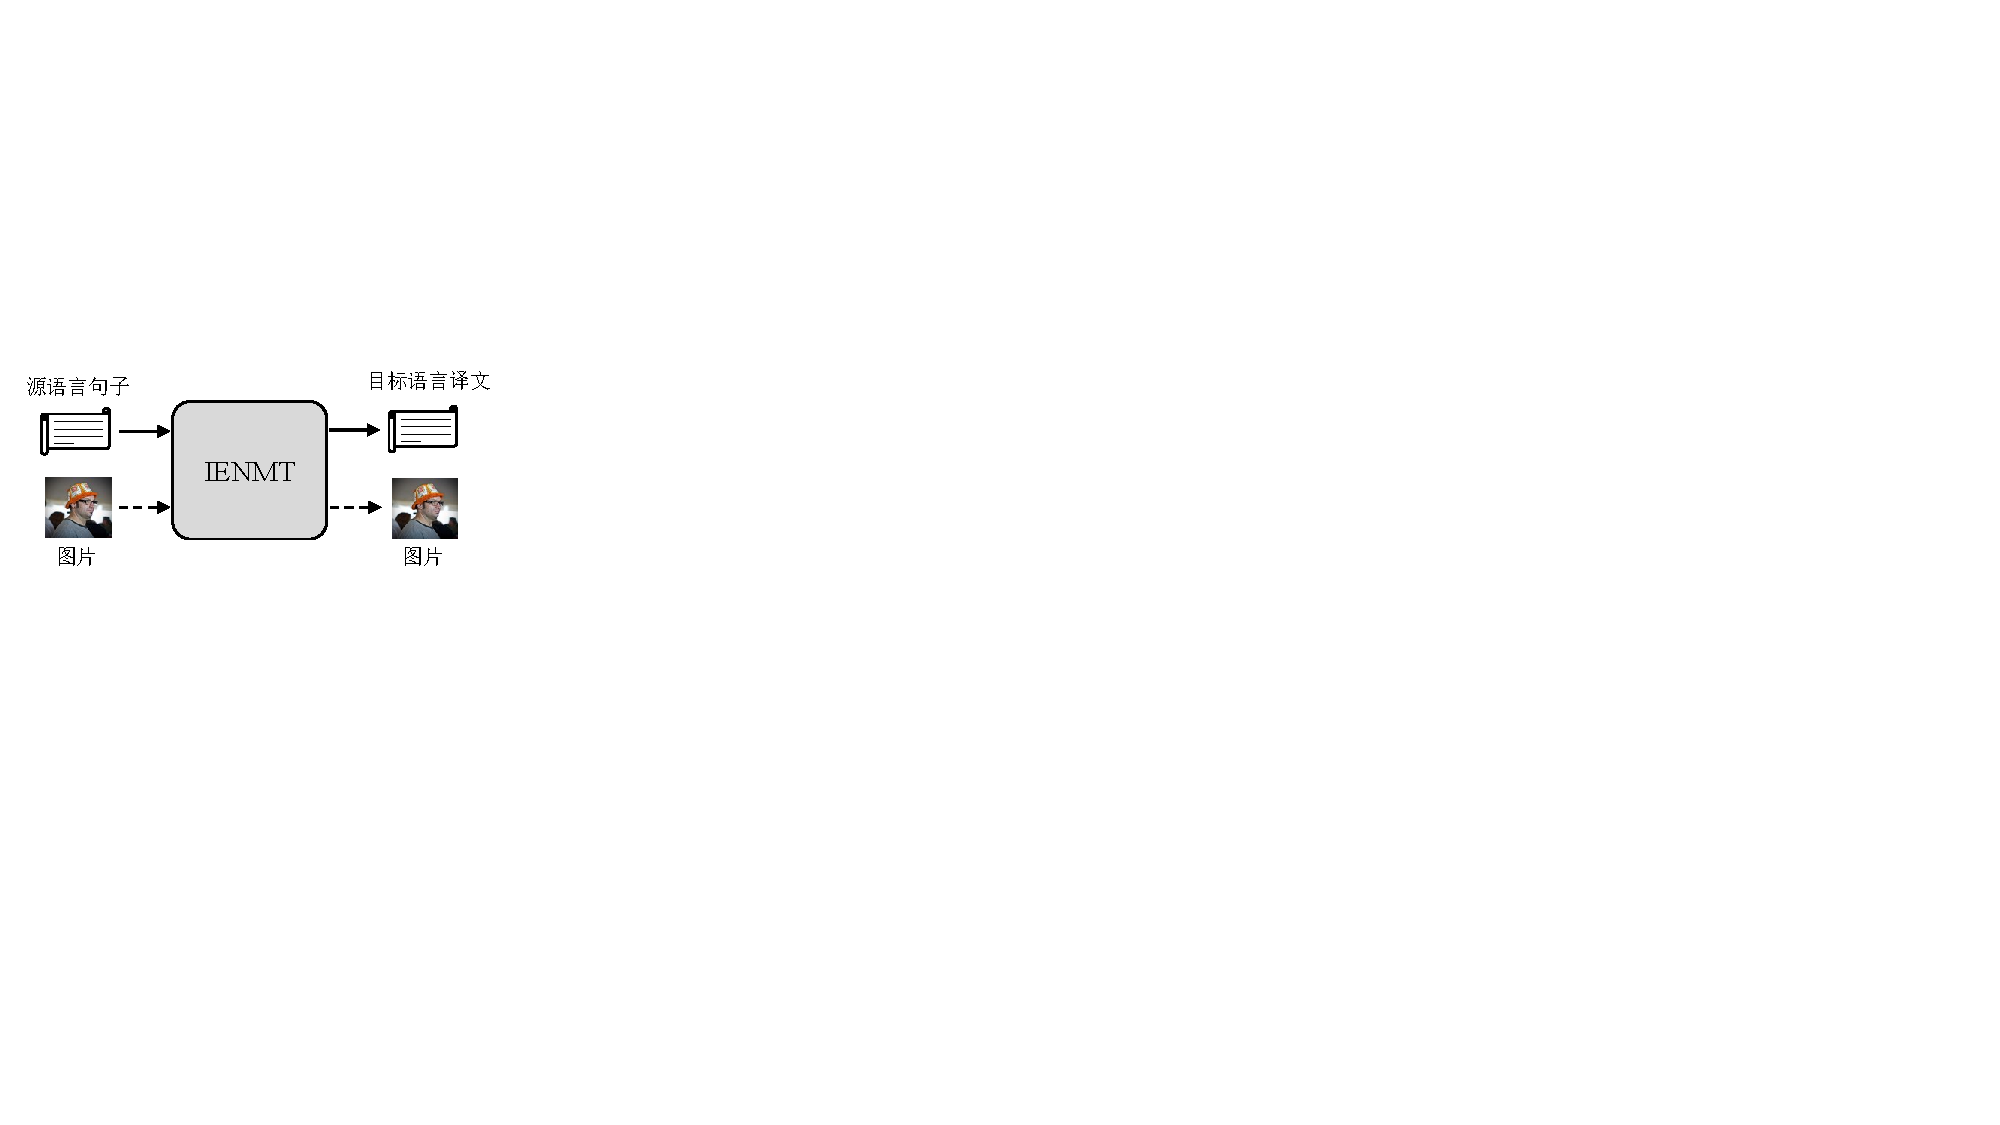
\includegraphics[width=\textwidth]{Img/fig_2_ienmt_train.pdf}
      \caption{训练阶段}
      \label{fig:2_ienmt_train}}
    \end{subfigure}%
    ~% line break
    \begin{subfigure}[b]{0.5\textwidth}
      \centering
      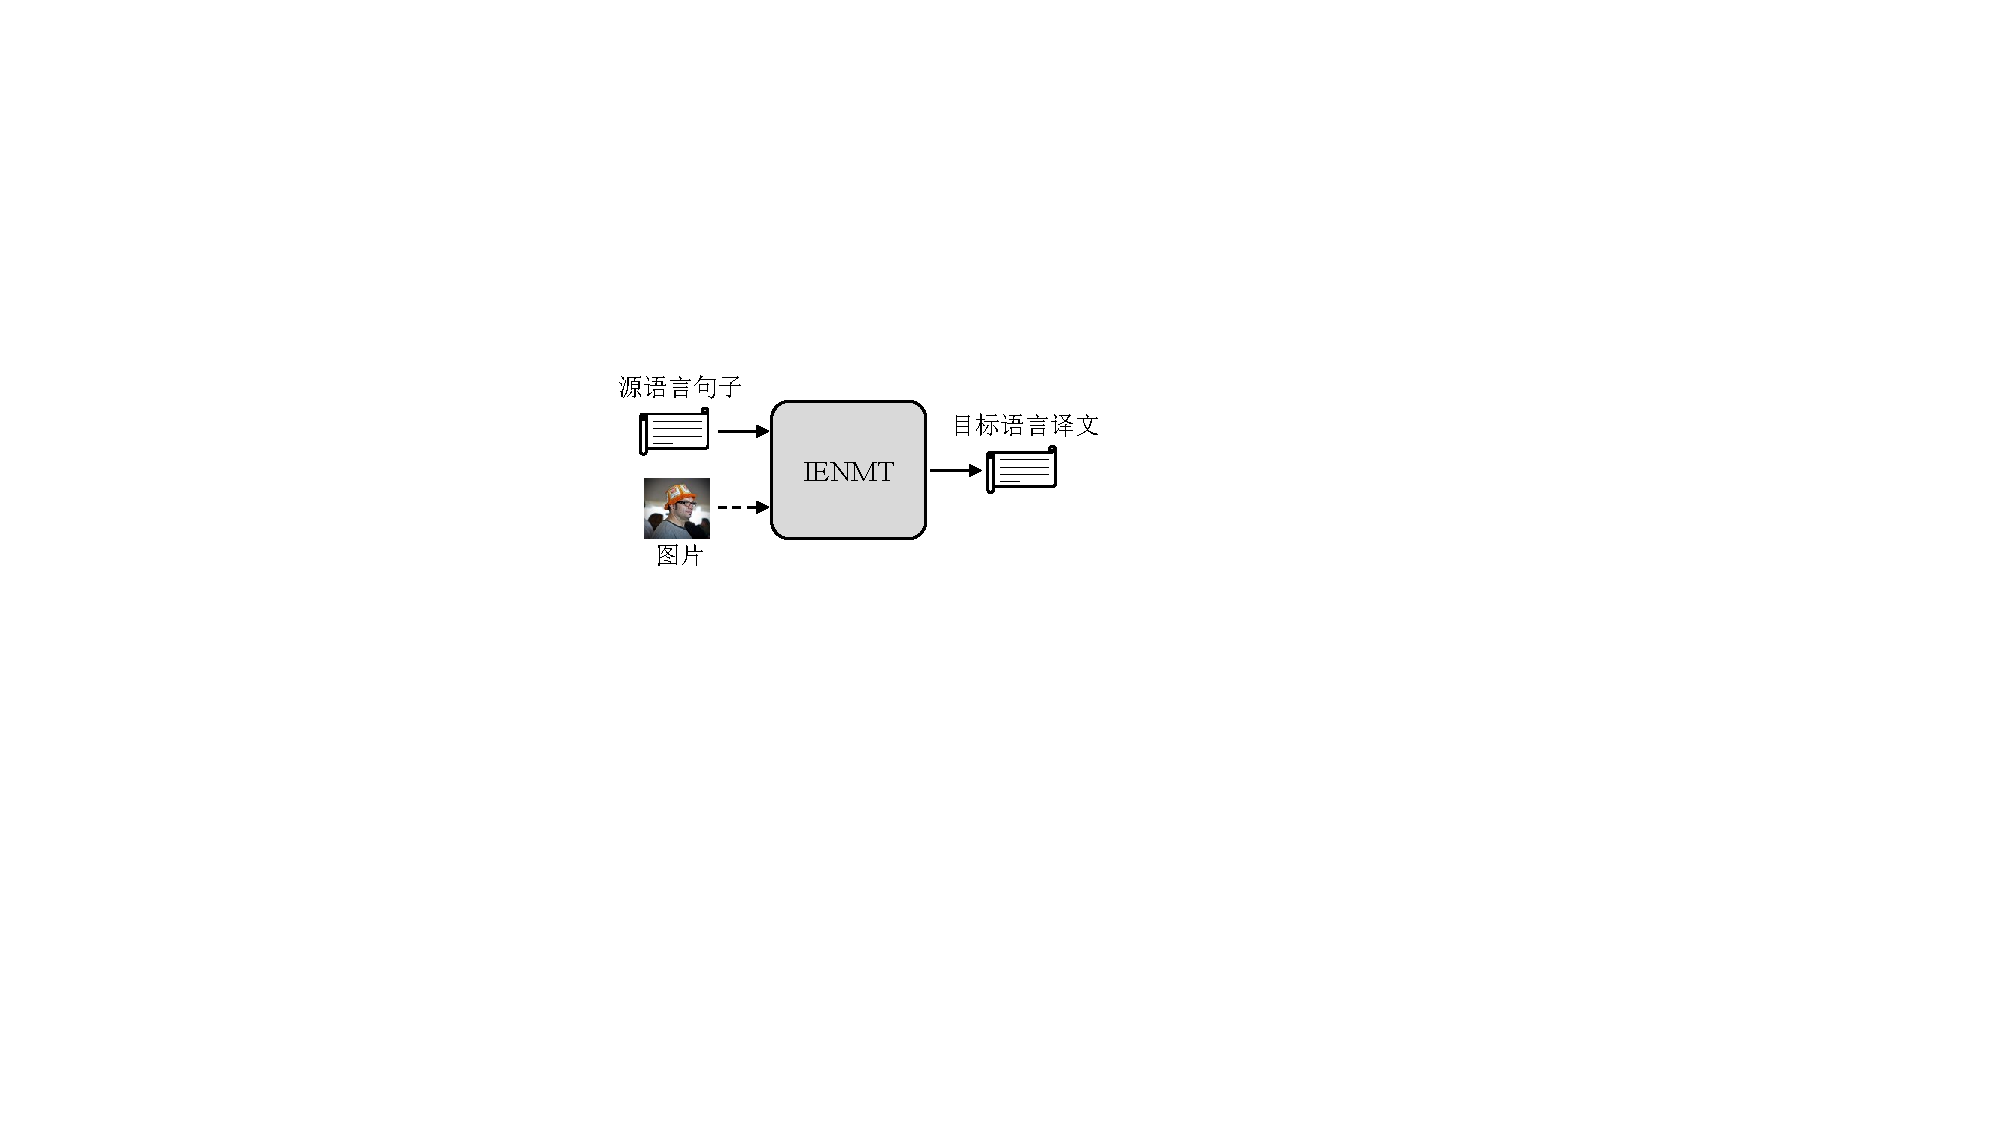
\includegraphics[width=\textwidth]{Img/fig_2_ienmt_infer.pdf}
      \caption{测试阶段}
      \label{fig:2_ienmt_infer}
    \end{subfigure}
    \bicaption{图片信息增强式神经机器翻译}{Image-enhanced neural machine translation}
    \label{fig:2_ienmt}
\end{figure}
上一节所述的图片信息辅助式神经机器翻译的主要特点是需要将图片输入到模型中,是模型利用视觉信息辅助整个翻译过程。期望通过这种方式解决待翻译文本中存在的多种病句问题,并且有大量的研究工作在这种方法范式上展开。然而,图片的作用方式不仅如此。图片信息增强式神经机器翻译(image-enhanced neural machine translation,IENMT)是一种利用特定的作用方式,将图片信息作用到模型的训练优化过程中,使神经机器翻译模型受益于这种优化方式,从而在翻译性能上得到进一步增强。图\ref{fig:2_ienmt}所示为根据目前已有的图片信息增强式神经机器翻译的相关工作总结得到的方法范式示意图。该方法的模型在训练和测试阶段的工作方式并不一致。在训练阶段,模型可以接收图片,也可以生成图片。不同的图片作用方式均有可能使模型受益。在测试阶段,模型可以是一个纯文本神经机器翻译模型,也可以融合图片信息。其工作方式主要取决于对优化过程的设计。

\tcite{kiros2014unifying,saha2016correlational,nakayama2017zero}在训练阶段将图片、源语言句子以及目标语言句子映射到一个统一的表示空间。这种方式试图将图片信息作为信息支点,然后通过将源语言和目标语言映射到这个支点,使文本的表示更忠于图片信息,从而提升纯文本翻译的质量。
\tcite{elliott2017imagination}提出了“想象力”机制。采用向量回归的方式难以得到一个统一的表示空间,因此通过文本表示“想象”一个与图片所包含的语义相近的图像特征,能够更准确的捕捉到图片中的语义。该方法将“想象力”机制与翻译通过多任务学习的方式优化一个纯文本的神经机器翻译模型,最终得到了稳定且显著的翻译质量提升。
\tcite{zhou2018visual}在“想象力”机制的基础上增加了视觉特征初始化解码器的方式,使图片信息不仅作用的模型性能的增强,还作用到翻译过程的解码辅助中。
\tcite{hirasawa2019multimodal}则增加预测预训练词向量来增强翻译模型。
\tcite{delbrouck2019adversarial}提出了图片重建的方法。与“想象力”机制不同的是,该方法应用生成对抗网络(generative adversarial network,GAN)将文本表示映射为完整的图片特征向量。这种图片生成方式进一步作用到翻译模型的优化增强中。

上述图片信息增强式神经机器翻译方法普遍利用了文本的编码表示生成目标图像的方法范式。而这种方法主要作用到模型的编码优化过程中,没有讨论是否有优化解码器的方案。本文第3章将对该问题做进一步的研究。
\subsection{基于图片搜索的神经机器翻译}
\begin{figure}[!htbp]
    \centering
    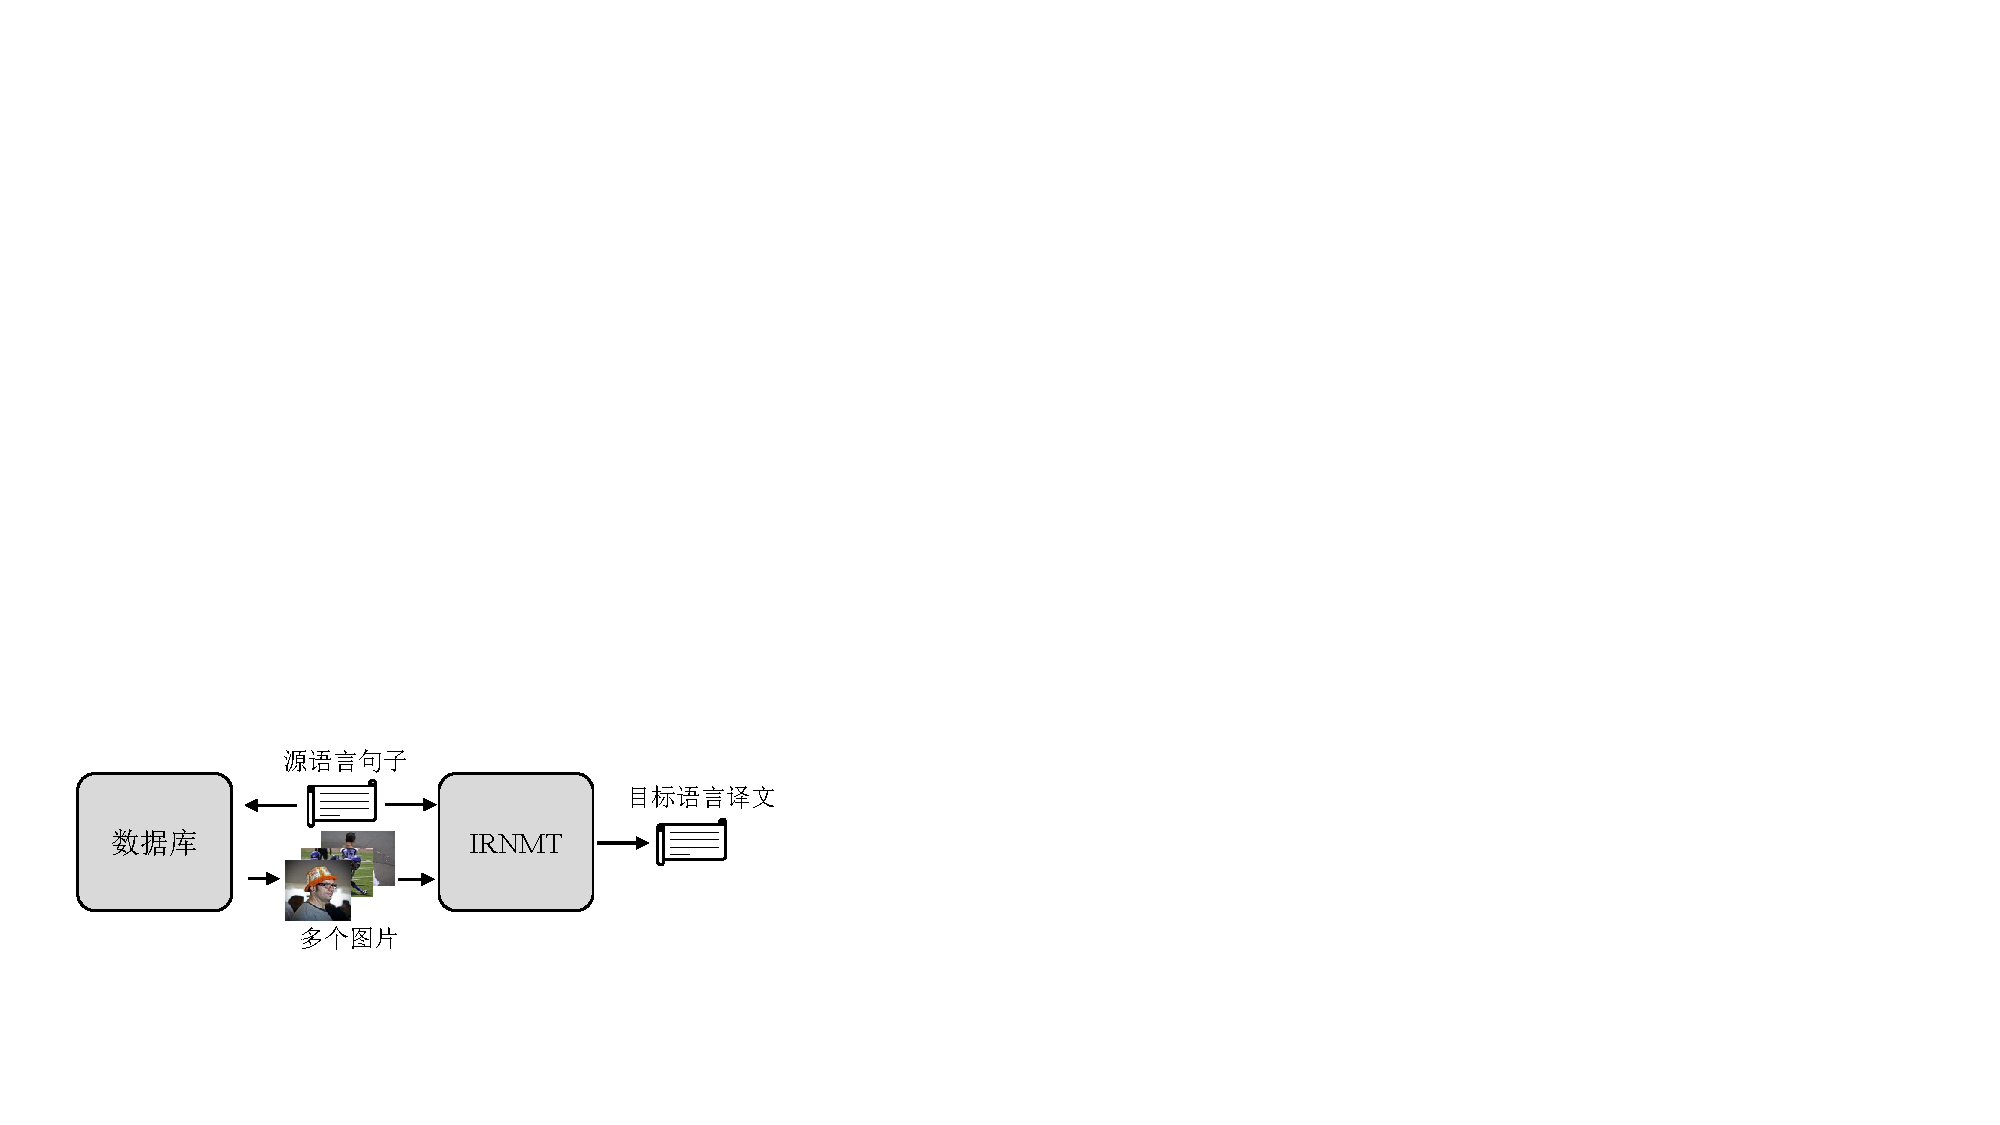
\includegraphics[scale=1]{Img/fig_2_irnmt.pdf}
    \bicaption{基于图片搜索的神经机器翻译}{Image-retrieval-based neural machine translation}
    \label{fig:2_irnmt}
\end{figure}
前两节所介绍的图片信息辅助式和图片信息增强式的神经机器翻译方法采用的都是与文本有着很强语义关系图片。因此,通常在图片描述的翻译任务上进行相关的研究与实验。本节的基于图片搜索的神经机器翻译(image-retrieval-based neural machine translation,IRNMT)与前面的方法区别在于该方法并不要求文本所描述的内容与图片内容完全一致。该方法采用与文本主题相关的搜索方法,从大规模单语语料或搜索引擎中收集相关图片。如图\ref{fig:2_irnmt}所示,为此类方法的研究范式示意图。文献\cite{118_DBLP:conf/iclr/0001C0USLZ20}首次提出在融合图片信息的神经机器翻译模型中增加搜索图片功能。该方法利用TF-IDF(term frequency-inverse document frequency)技术建立一个单词到图片的查找表,从这个查找表中可以获得图片的相关主题信息。在进行图片搜索之前,需要从源语言句子中提取出与句子内容相关的主题单词,然后根据主题搜索出若干个与该主题最相关的图片以此来获得所需要的图片信息。然后将这些图片的特征提取出来,最后传递给神经机器翻译模型用于辅助翻译生成。文献\cite{20_wu-etal-2021-good}在以上基于图片搜索的方法中测试图片信息是否能够为翻译带来提升。文献\cite{119_fang-feng-2022-neural}为了在搜索到更相关的图片,为翻译提供更准确的视觉信息,采用短语级别的图片作用方式,在搜索到图片后,需要提取出与主题相关的视觉目标,然后再进一步地在翻译中融合图片信息。
文献\cite{120_tang-etal-2022-multimodal}为了增加图片搜索的资源,并且使相关方法能够受益于一般的文本翻译任务,采用了基于商用搜索引擎的方案。

目前基于图片搜索的神经机器翻译方法的相关研究还处在初步阶段,基于搜索的方法的相关研究也在问答系统\cite{121_DBLP:conf/icml/GuuLTPC20}、对话系统\cite{122_DBLP:conf/emnlp/WestonDM18}、语言模型\cite{123_DBLP:conf/iclr/KhandelwalLJZL20}以及纯文本翻译\cite{124_DBLP:conf/aaai/GuWCL18}等任务中得到了应用。然而这类方法还存在着诸多问题需要进一步地解决,例如文本主题提取的准确性与覆盖性对图片搜索的影响,搜索获得图片与文本翻译内容的相关性对翻译带来的影响。
%这部分要强调使用完全对应图片的方案都很难使视觉信息起作用,那么采用搜索式的方式就更难了
%方法范式:与前面方法的最大不同点是否图文对应
%举例
%优点
%缺点

\subsection{基于图片信息的无监督神经机器翻译}
\begin{figure}[!htbp]
    \centering
    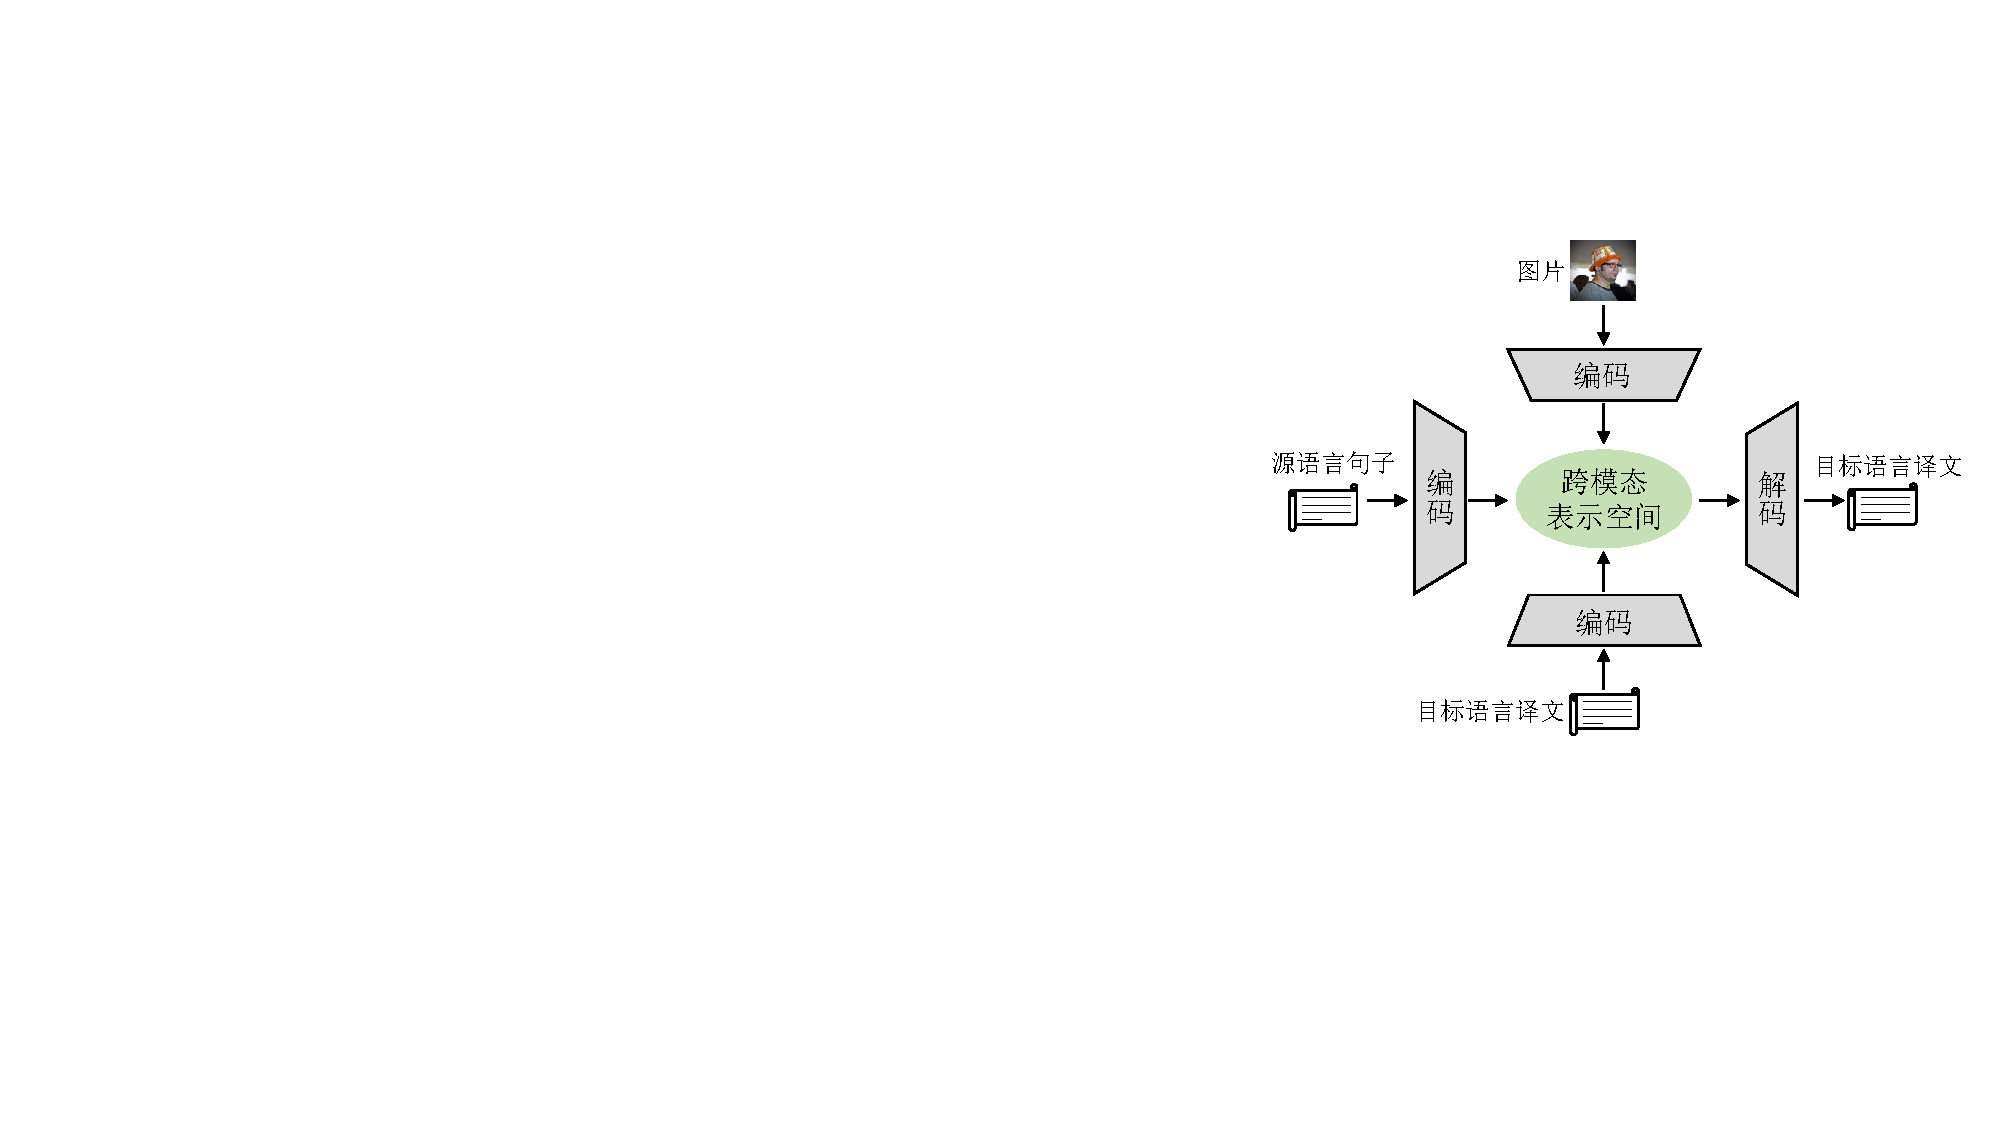
\includegraphics[scale=1]{Img/fig_2_iunmt.pdf}
    \bicaption{基于图片信息的无监督神经机器翻译}{Image-based unsupervised neural machine translation}
    \label{fig:2_iunmt}
\end{figure}
基于图片信息的无监督神经机器翻译(image-based unsupervised neural machine translation,IUNMT)是指利用图片作为语言桥梁,为零资源的翻译提供翻译支持的一类方法。零资源语言的翻译问题通常选择一个中间语言作为桥梁,通过将源语言翻译到中间语言,再将中间语言翻译到目标语言的方式,解决源语言到目标语言的翻译问题。然而,这种方法仍然需要源语言和目标语言到中间语言的平行翻译数据,而很多的低资源语言之间的翻译很难通过这种办法解决。考虑到人的语言可能分为多种,但人眼中的世界是统一的,并且社交媒体中包含了大量的单语的图文数据,所以选择视觉模态作为中间语言来完成零资源机器翻译任务是一个很好的选择。
文献\cite{115_saha-etal-2016-correlational}采用了中间语言方案解决源语言与目标语言之间没有平行的训练数据的问题。该方法选择图片作为中间语言,通过联合训练源语言到图片和图片到目标语言的生成模型,最终过得源语言到目标语言的翻译模型。
文献\cite{54_DBLP:journals/mt/NakayamaN17}同样将图片作为了中间语言,在训练过程中,将源语言、目标语言、和图片映射到一个统一的跨模态表示空间。
文献\cite{125_DBLP:conf/aaai/ChenLL18}将零资源的神经机器翻译模型的训练过程构建为一个多智能体交流游戏(multi-agent communication game)。每个智能体分别负责从图片中生成描述,以及从描述中生成目标语言译文的任务。两个智能体在两种任务的配合下完成源语言到目标语言的翻译建模。
文献\cite{126_DBLP:conf/cvpr/SuFBKH19}采用降噪模型的训练方式构建中间语言与源语言和目标语言的编码器和解码器,在联合使用编码器和解码器的情况下实现源语言到目标语言之间的翻译。
文献\cite{55_DBLP:conf/ijcai/ChenJF19}认为图片中包含太多与待翻译句子以及译文不相关信息,直接作为句子级语义单位的中间语言会引入大量噪音,因此将图片先应用到词的翻译,在通过迭代生成伪平行句对的方式,逐步实现句子级的翻译。
文献\cite{127_huang-etal-2020-unsupervised-multimodal}同样通过图片生成伪平行句对的方式逐步训练翻译模型。




%\section{图片信息辅助式神经机器翻译}
得益于神经网络方法的快速发展,自然语言文本与图片的信息融合成为了可能。融入图片信息的机器翻译的研究历程也紧随着纯文本的神经机器翻译的脚步而发展。然而,相关研究则最早起源于图像描述生成任务。有部分学者将文本作为一个外源信息来辅助图片描述的生成,但这种方式的本质则是在翻译任务中融入视觉信息。2016年WMT将多模态机器翻译引入作为共享任务后,MMT受到了广泛的关注。在之后的WMT17和WMT18,MMT任务延续并奠定了在机器翻译中融合图片信息作为多模态机器翻译研究的主要范式。

%平行翻译句一般具有良好的对齐特性,这使得融入的外源信息仅用于辅助少数具有歧义、信息不完整以及训练不充分等问题的句子的翻译。该特性也成为了展开相关研究道路上的一大难点。
融合图片信息的神经机器翻译任务主要采用的是平行翻译句对加图片三元组形式的数据,即一张图片对应一句描述和一句翻译。大部分相关研究需要对神经机器翻译模型进行适当的修改,以适应图片的输入。模型中输入的图片可用于辅助优化翻译过程中源语言的语义表示,或为解码过程增加辅助外源信息。本文将这种在翻译过程中以源端文本作为信息主体,输入图片用于语义信息强化的方法称为图片信息辅助式神经机器翻译。可根据图片信息融合到翻译模型中的方式将这种方法分为三类:融合图片全局信息、融合图片局部动态信息以及融合图片视觉目标信息。这些三种图片信息以视觉特征为载体输入到翻译模型中,视觉特征则是从预训练的卷积神经网络中提取得到。不同的提取方式所包含的语义信息的粒度和特征维度有所不同。将这些不同形式的视觉特征整合到NMT模型后,模型进行跨模态语义融合的难易程度则取决于模型设计的合理性。

\subsection{融合图片全局信息的神经机器翻译}

\cite{18_DBLP:conf/emnlp/CalixtoL17}
\cite{19_DBLP:conf/acl/CalixtoRA19}
\cite{20_DBLP:conf/acl/WuKBLK20}


\subsection{融合图片局部动态信息的神经机器翻译}

\subsection{融合图片视觉目标信息的神经机器翻译}



%% 2.4 visual enhanced MMT
%\section{图片信息增强式神经机器翻译}
%% 2.5 retrieval-based MMT
%\section{基于图片搜索的神经机器翻译}





\section{问题分析与总结}
% 还要几篇分析性质的工作
% MMT的演变与拥有的优势
% MMT现有存在的问题
从基于循环神经网络的RNMT,到目前广泛采用的Transformer,研究者们致力于将图片中的视觉信息以各种方式融合到翻译过程中,从而提升机器翻译的质量。这是因为,相比于纯文本,图片中往往包含更完整、更细节以及更丰富的语义信息。然而,相比于纯文本翻译利用端到端模型就可以学习到跨语言的表示与生成,融入图片信息的神经机器翻译并不是简单地将图片输入到模型中就能够将跨模态的信息进行融合并利用。

得益于不同模态的信息在神经网络方法中普遍以分布式向量表示的形式呈现,在神经翻译模型中实现跨模态信息融合具有很强的优势:1)能够直接从数据中学习数据特征,不需要人为的特征设计;2)采用成熟的神经翻译模型作为主框架,采用预训练的卷积神经网络用于图片编码,跨模态信息融合可以在现有模型基础上进行改进;3)图片作为上下文信息的表示方法与融合方式,和一般的文档上下文或视频上下文类似,相应的模型方法有很强的泛化复用性;4)解决歧义词或语义不完整等文本中出现信息缺失或语病等问题。

相比于基于图片搜索的神经机器翻译和基于图片信息的无监督神经机器翻译,图片信息辅助式和图片信息增强式的方法更符合融合图片信息的神经机器翻译方法的实际应用场景。因此本文将主要围绕这两类方法展开研究工作。
基于对这两类方法的总结,本文还将相关方法分为显式和隐式两类跨模态信息融合方法。显式跨模态信息融合方法将图片信息直接作用到与图片内容相关的文本语义单元上。隐式跨模态信息融合方法直接将图片输入给翻译模型,利用神经网络方法能够直接从数据中学习特征的优点将文本信息与图片信息相融合。
显式方法能够将图片信息更明确地作用到翻译中,使图片信息更容易为模型所利用,但却需要为模型提供图片与文本的显式对齐关系,很少有工作在此类方法上面展开研究。隐式方法的优点在于模型设计简单,主要利用了神经网络方法针对不模态信息建模的共性,因此更受广大研究者的关注,成为了目前的主流方法。
% 本文索要解决的问题:三篇文章
然而,隐式方法却存在一些问题,例如输入图片信息的方式不一定有效,图片信息的作用方式不明确,翻译模型对视觉信息不敏感等问题。尽管当前广泛应用的神经翻译模型与计算机视觉基础模型为跨模态信息融合提供了极大的便利,依旧难以针对不同跨模态信息需求的文本翻译数据设计统一的模型方案。为此,本文尝试回答三个问题:
\begin{itemize}
    % 输入图片不一定带来提升
    \item {\sffamily 图片信息的有效性}。相关工作的实验表明,相比于纯文本神经机器翻译,输入图片信息后的翻译模型的翻译准确率并没有得到明显的提升,有些甚至会低于纯文本翻译\pcite{duttachowdhury2019understanding,li2021vision,wu2021good}。这说明在一般的机器翻译模型中,图片信息与文本信息的融合并不是一个必然的过程。如何使融合图片信息的神经机器翻译获得有效的翻译准确率的提升?
    % 隐含式方法的弊端
    \item {\sffamily 图片信息作用方式不明确}。尽管已有很多模型方法表明输入图片信息能够为翻译质量带来提升,然而图片信息的作用方式并不明确。例如,歧义词问题是否得到解决?语义不完整的句子是否得到补全?亦或是在其它不得而知的方面为翻译带来了增益?那么如何利用显示跨模态信息融合方法将图片信息作用到神经翻译中?
    % 输入噪音可能比输入图片带来的提升更多
    \item {\sffamily 翻译模型对视觉信息不敏感}。\tcite{elliott2018adversarial}将与文本内容不一致的图片输入到翻译模型中来测试模型翻译准确率的提升是否来自于图片中的视觉信息,实验结果显示大部分模型可以从错误的图像中获得同样或相近的翻译准确率的提升。\tcite{wu2021good}认为输入图片与输入噪音的作用相似,是正则化作用而非视觉信息为模型带来的翻译准确率的提升。如何使翻译模型对输入图片信息敏感?
\end{itemize}

为此,本文围绕融合图片信息的神经机器翻译方法研究,从改进模型的训练方式、图片的输入方式、视觉信息的作用方式等方面展开研究工作:
\begin{itemize}
    % 翻译质量提升不稳定,作用方式不明确
    \item {\sffamily 基于跨模态文本重构的神经机器翻译:}为解决图片信息作用方式不明确的问题,提出了一种基于显式跨模态信息融合方法的图片增强式神经机器翻译。该方法改变了图片的输入方式,使用图片的视觉目标特征以替换的方式作用到词或短语两种粒度上,用于重构完整的文本。然后改变了模型的训练方式,以多任务训练的方式,利用跨模态的文本重构任务优化神经机器翻译模型的表示能力,从而提升翻译的准确率,使模型能够有效利用图片信息。第3章将介绍本文提出的基于跨模态文本重构的神经机器翻译方法。
    % 翻译质量提升不稳定,作用方式不明确
    \item {\sffamily 基于双向跨模态实体重构的神经机器翻译:}在上一部分工作的基础上,结合显式和隐式两种跨模态信息融合方法。以明确的方式,针对文本实体和视觉实体实现双向跨模态实体重构。针对非实体词,使用文本上下文与视觉实体组合而成的跨模态上下文生成文本非实体。该方法不再重构完整的文本,针对实体级的重构方法即可得到更好的模型结果。第4章将介绍本文提出的基于双向跨模态实体重构的神经机器翻译方法。
    % 翻译质量提升不稳定,对视觉信息不敏感
    \item {\sffamily 基于图文对比对抗训练的神经机器翻译:}在训练图片信息辅助式的神经翻译模型的同时,采用对比学习方法学习译文与多模态输入的联合语义表示空间。为了解决模型对视觉信息不敏感的问题,在对比学习的负样本集中加入图文不一致的对抗样本。通过提升翻译模型区分输入图片正确与否的能力,强迫模型将图片中的视觉信息融合到文本表示中,从而强化源端文本的特征表示,实现翻译准确率的提升,使翻译模型在测试阶段也能有效利用图片信息。第5章将介绍本文提出的基于图文对比对抗训练的神经机器翻译方法。
\end{itemize}
%(在这里提到模型对视觉信息不敏感的问题,然后循序渐进讲为什么我们的研究以增强式为主,后又如何补充辅助式)



\section{本章小结}
本章介绍了与融合图片信息的神经机器翻译相关的国内外研究,其中包括神经机器翻译主流模型的发展过程和计算机视觉相关的基础模型。然后主要介绍了在神经翻译模型中融合图片信息的主流方法,以及各类方法所具备的特点。本章分析了现有融合图片信息的神经机器翻译方法的缺陷,简要地说明了相应的解决办法,以及针对这些问题本文的一些应对思路。这些内容与本文的研究内容息息相关,在后面的章节中,本文将针对如何有效地将图片中的视觉信息融合到神经翻译模型中给出相应的解决方案。

